\section{Autonomous Walking}
\label{sec::52_aw}
The autonomous walking is based upon the performance within the test environment from section \ref{sec::512_pt}. The found parameters are used for comparative reason throughout this section as well. As explained in section \ref{sec::324_ip}, the neural network benefits strongly from an available depth map as input. We will therefore deal with the depth map extraction first.
\subsection{Camera Calibration}
As described in section \ref{sec::324_ip}, in order for the stereo block matching algorithm to work properly (equation \ref{eq::324_sad}), it is required to calibrate the cameras. We shortly verified this in figure \ref{fig::521_no_calib}, where we extracted a depth map from the uncalibrated stereo camera pair.
\begin{figure}[h]
	\centering
	\subcaptionbox{Left disparity map.}%
	[.4\linewidth]{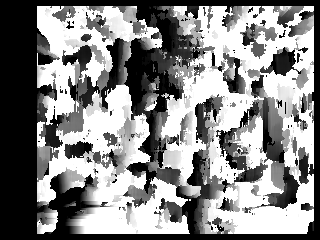
\includegraphics[scale=.3]{chapters/05_experiments/02_autonomous_walking/02_depth_map_parameter_tuning/disp_no_calib.png}}
	\subcaptionbox{Confidence weighted least squares filtered disparity map.}%
	[.4\linewidth]{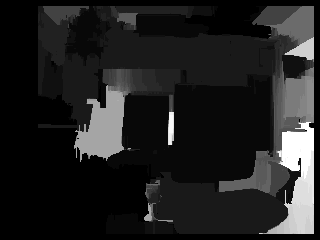
\includegraphics[scale=.3]{chapters/05_experiments/02_autonomous_walking/02_depth_map_parameter_tuning/wls_no_calib.png}}
	\caption{Depth map extraction without calibration. The parameters were set as follows to $N=13$, $D=32$, $\sigma = 1$, and $\lambda=10^4$.}
	\label{fig::521_no_calib}
\end{figure}
For the calibration we chose to use a chess-board calibration pattern, see figure \ref{fig::521_calib}. The used calibration pattern has width of $W=8$, and a height of $H=6$, where each square has a size of $a=22.5\,\text{mm}$ (equation \ref{eq::324_square_size}). We took a total of $N=60$ images of the calibration pattern for varying orientations and translations with respect to the camera, which results in a total of $W\times H\times N = 2880$ points for the calibration. 
\begin{figure}[h]
	\centering
	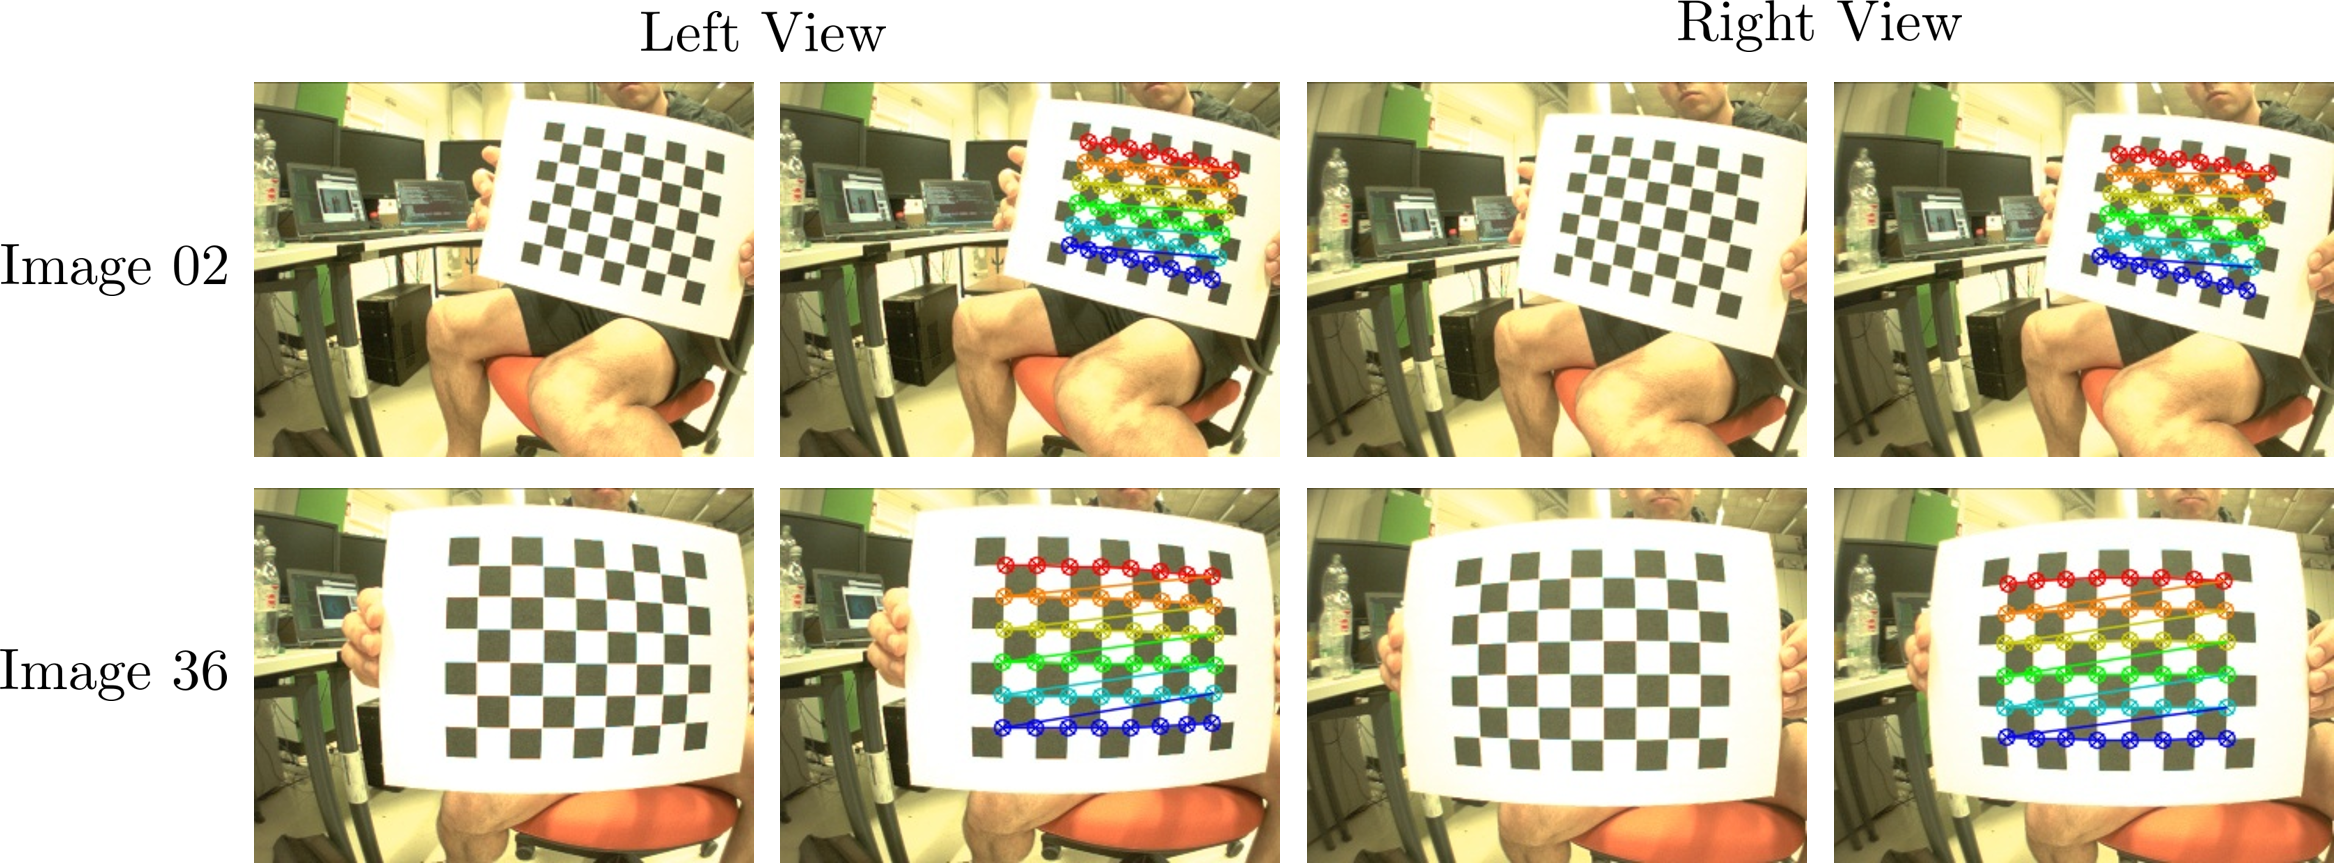
\includegraphics[scale=.28]{chapters/05_experiments/02_autonomous_walking/01_camera_calibration/calib.png}
	\caption{Exemplary left and right camera views of the calibration pattern as acquired during the calibration process. The colorful points indicate the detected corners in the image plane. Refer to figure \ref{fig::324_distortion} for the theory.}
	\label{fig::521_calib}
\end{figure}
As the resulting mean squared re-projection error $\Delta \bar{x} = 1/(WHN)\sum_0^{WHN} \Delta x$ (equation \ref{eq::324_reprojection}), we obtained $\Delta \bar{x}_l = 0.26\, \text{pixel}$, and $\Delta \bar{x}_r = 0.25\,\text{pixel}$, for the left, and the right camera, respectively. According to equations \ref{eq::324_focal_intrinsics}, \ref{eq::324_x_dist}, and \ref{eq::324_y_dist}, we therefore determined the camera intrinsic parameters as listed in table \ref{tab::521_intrinsics}.
\begin{table}[h]
	\centering
	\begin{tabular}{lll}
		Intrinsic Parameter & Left Camera & Right Camera\\
		\hline
		$f_x\,[\text{pixel}/\text{mm}]$ & $\quad2.36\cdot10^2$ & $\quad2.32\cdot10^2$ \\
		$f_y\,[\text{pixel}/\text{mm}]$ & $\quad2.37\cdot10^2$ & $\quad2.32\cdot10^2$ \\
		$c_x\,[\text{pixel}]$ & $\quad1.63\cdot10^2$ & $\quad1.86\cdot10^2$ \\
		$c_y\,[\text{pixel}]$ & $\quad1.11\cdot10^2$ & $\quad1.30\cdot10^2$ \\
		$k_1\,[1/\text{pixel}^2]$ & $-4.54\cdot10^{-1}$ & $-4.58\cdot10^{-1}$ \\
		$k_2\,[1/\text{pixel}^4]$ & $\quad2.90\cdot10^{-1}$  & $\quad3.18\cdot10^{-1}$  \\
		$k_3\,[1/\text{pixel}^6]$ & $-1.21\cdot10^{-1}$ & $-1.48\cdot10^{-1}$ \\
		$p_1\,[1/\text{pixel}]$ & $-2.73\cdot10^{-3}$ & $\quad3.02\cdot10^{-4}$  \\
		$p_2\,[1/\text{pixel}]$ & $\quad2.16\cdot10^{-4}$  & $\quad7.63\cdot10^{-4}$		
	\end{tabular}
	\caption{Intrinsic parameters of single cameras. These parameters can be found as YAML file on GitHub (\href{https://github.com/mhubii/nmpc_pattern_generator/tree/master/libs/io_module}{link}).\label{tab::521_intrinsics}}
\end{table}
Then given the calibration of each single camera, we computed the rectification transforms $\bm{R}_i$, and the projection matrices $\bm{P}_i$ in the rectified coordinate system for each camera \ref{tab::521_extrinsics}.
\begin{table}[h]
	\centering
	\begin{tabular}{lll}
		Camera & Extrinsic Parameter & \\ 
		\hline
		&& \\
		\multirow{5}{*}{Left} & $\bm{R}\,[\text{a.u.}]$              & $\begin{pmatrix}
		\quad9.93\cdot10^{-1} & -2.65\cdot10^{-3}     & \quad1.14\cdot10^{-1} \\ 
		\quad5.41\cdot10^{-1} & \quad1.00\cdot10^{0}  & -2.39\cdot10^{-2} \\
		-1.14\cdot10^{-1}     & \quad2.43\cdot10^{-2} & \quad9.93\cdot10^{-1}
		\end{pmatrix}$ \\&&\\
		& $\bm{P}\,[\text{pixel}/\text{mm}]$              & $\begin{pmatrix}
		2.34\cdot10^{2} & 0.00     & 1.88\cdot10^{2} & 0.00\,\text{mm} \\ 
		0.00 & 2.34\cdot10^{2}  & 4.87\cdot10^{1} & 0.00\,\text{mm} \\
		0.00    & 0.00 & 1.00 & 0.00\,\text{mm}
		\end{pmatrix}$ \\
		&&\\
		\multirow{5}{*}{Right} & $\bm{R}\,[\text{a.u.}]$              & $\begin{pmatrix}
		\quad9.95\cdot10^{-1} & -2.30\cdot10^{-2}     & \quad9.93\cdot10^{-2} \\ 
		\quad2.07\cdot10^{-2} & \quad1.00\cdot10^{0}  & \quad2.38\cdot10^{-2} \\
		-9.98\cdot10^{-2}     & -2.16\cdot10^{-2} & \quad9.95\cdot10^{-1}
		\end{pmatrix}$ \\&&\\
		& $\bm{P}\,[\text{pixel}/\text{mm}]$              & $\begin{pmatrix}
		2.34\cdot10^{2} & 0.00     & 1.88\cdot10^{2} & -1.60\cdot10^1\,\text{mm} \\ 
		0.00 & 2.34\cdot10^{2}  & 4.88\cdot10^{1} & 0.00\,\text{mm} \\
		0.00    & 0.00 & 1.00 & 0.00\,\text{mm}
		\end{pmatrix}$ \\
	\end{tabular}
	\caption{Rectification transforms $\bm{R}_i$, and projection matrices $\bm{P}_i$, for the left, and the right camera, respectively. These parameters can be found as YAML file on GitHub (\href{https://github.com/mhubii/nmpc_pattern_generator/blob/master/libs/io_module/cam_stereo.yaml}{link}). \label{tab::521_extrinsics}}
\end{table}
Exemplary rectified images, which rely on the matrices of table \ref{tab::521_extrinsics}, are shown in figure \ref{fig::521_rect} (a). Since there is a slight rotation of the calibration pattern, it is not obvious that the images got rectified well. Therefore, the same images are shown in figure \ref{fig::521_rect} (b), but slightly rotated such that the calibration pattern aligns horizontally. The blue line therein indicates that in contrast to the original image, straight lines now appear straight across both images, which is crucial for the block matching algorithm in the next section - Depth Map Parameter Tuning.
\begin{figure}[h]
	\centering
	\subcaptionbox{Rectified images.}%
	[.4\linewidth]{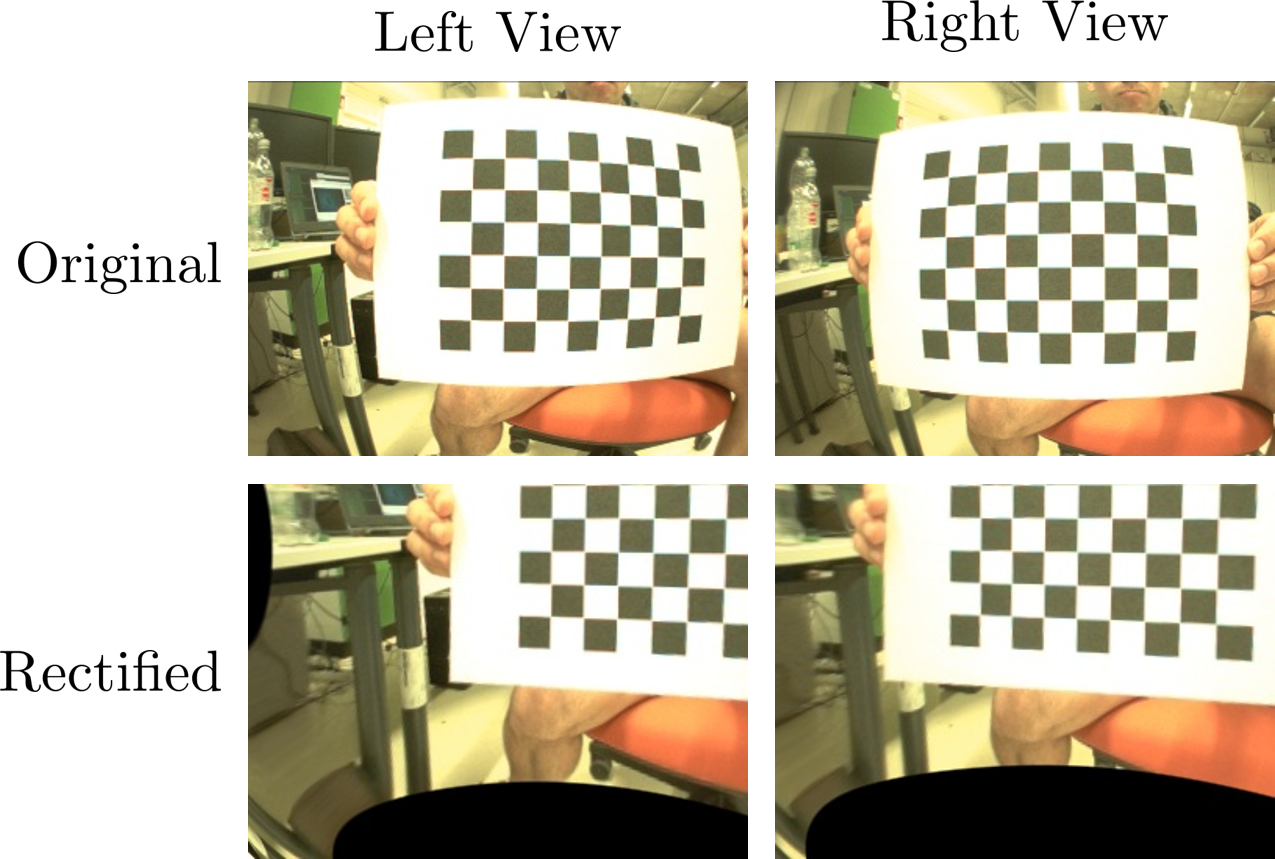
\includegraphics[scale=.25]{chapters/05_experiments/02_autonomous_walking/01_camera_calibration/rect.png}}
	\subcaptionbox{Rotated rectified images.}%
	[.4\linewidth]{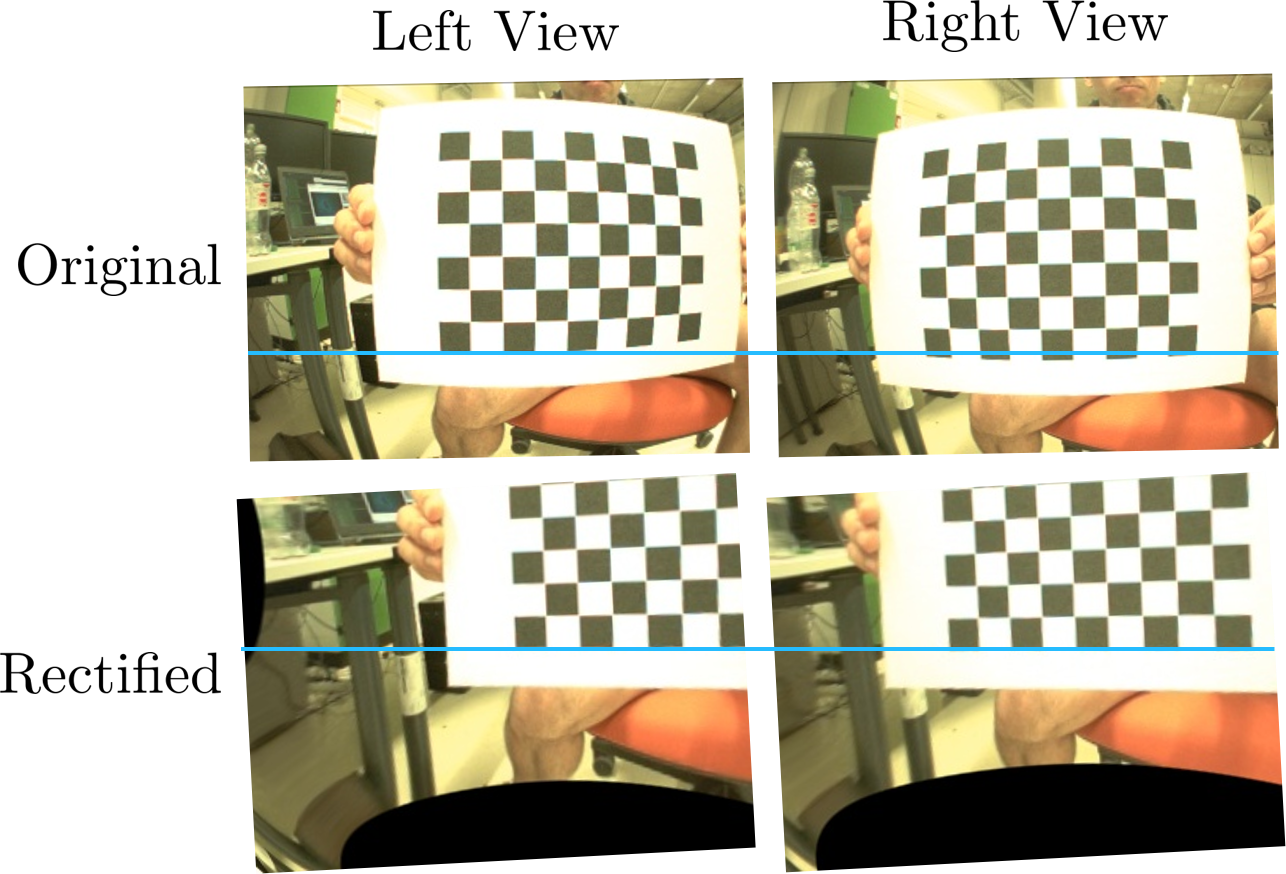
\includegraphics[scale=.25]{chapters/05_experiments/02_autonomous_walking/01_camera_calibration/rect_line.png}}
	\caption{Rectified and original view of the stereo camera. Refer to figure \ref{fig::324_rectified} for the theory.}
	\label{fig::521_rect}
\end{figure}
\subsection{Depth Parameter Tuning}
Within this section, we shortly explore the effects of all tunable parameters on the depth map generation. Therefore, we utilize a simple experimental setup. Within the setup, Heicub points its stereo camera towards three chairs that are located at a distance of $1\,\text{m}$ towards each other, and towards the cameras, so to cover close, medium, and far distances. The consecutive chairs are slightly shifted, in order to enable the simultaneous observation of all of them. The rectified view of the environment is shown in figure \ref{fig::522_wls_rgb}.
\begin{figure}[h]
	\centering
	\subcaptionbox{Left camera's view.}%
	[.4\linewidth]{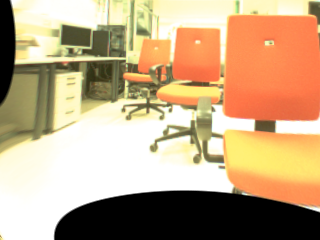
\includegraphics[scale=.3]{chapters/05_experiments/02_autonomous_walking/02_depth_map_parameter_tuning/l_rgb.png}}
	\subcaptionbox{Right camera's view.}%
	[.4\linewidth]{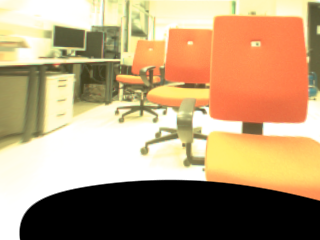
\includegraphics[scale=.3]{chapters/05_experiments/02_autonomous_walking/02_depth_map_parameter_tuning/r_rgb.png}}
	\caption{Heicub's perspective of the scene for the depth map parameter tuning.}
	\label{fig::522_wls_rgb}
\end{figure}
The depth map extraction, which utilizes the rectified images, depends on a stereo block matching algorithm that got explained in section \ref{sec::324_ip}. It mainly depends on the window size and the number of disparities for the sum of absolute difference computation. We evaluate the influence of those two parameters in figure \ref{fig::522_disp} (a) in a grid search fashion. It is apparent that the change in the number of disparities has close to no influence onto the depth map quality, while it removes plenty of useful information from the left hand side of images. The same holds true for the window size, except that it removes some noise from the depth maps.
\begin{figure}[h]
	\centering
	\subcaptionbox{Left disparity. Please refer to figure \ref{fig::324_left_disparity_map} and equation \ref{eq::324_sad} for the theory.}%
	[.45\linewidth]{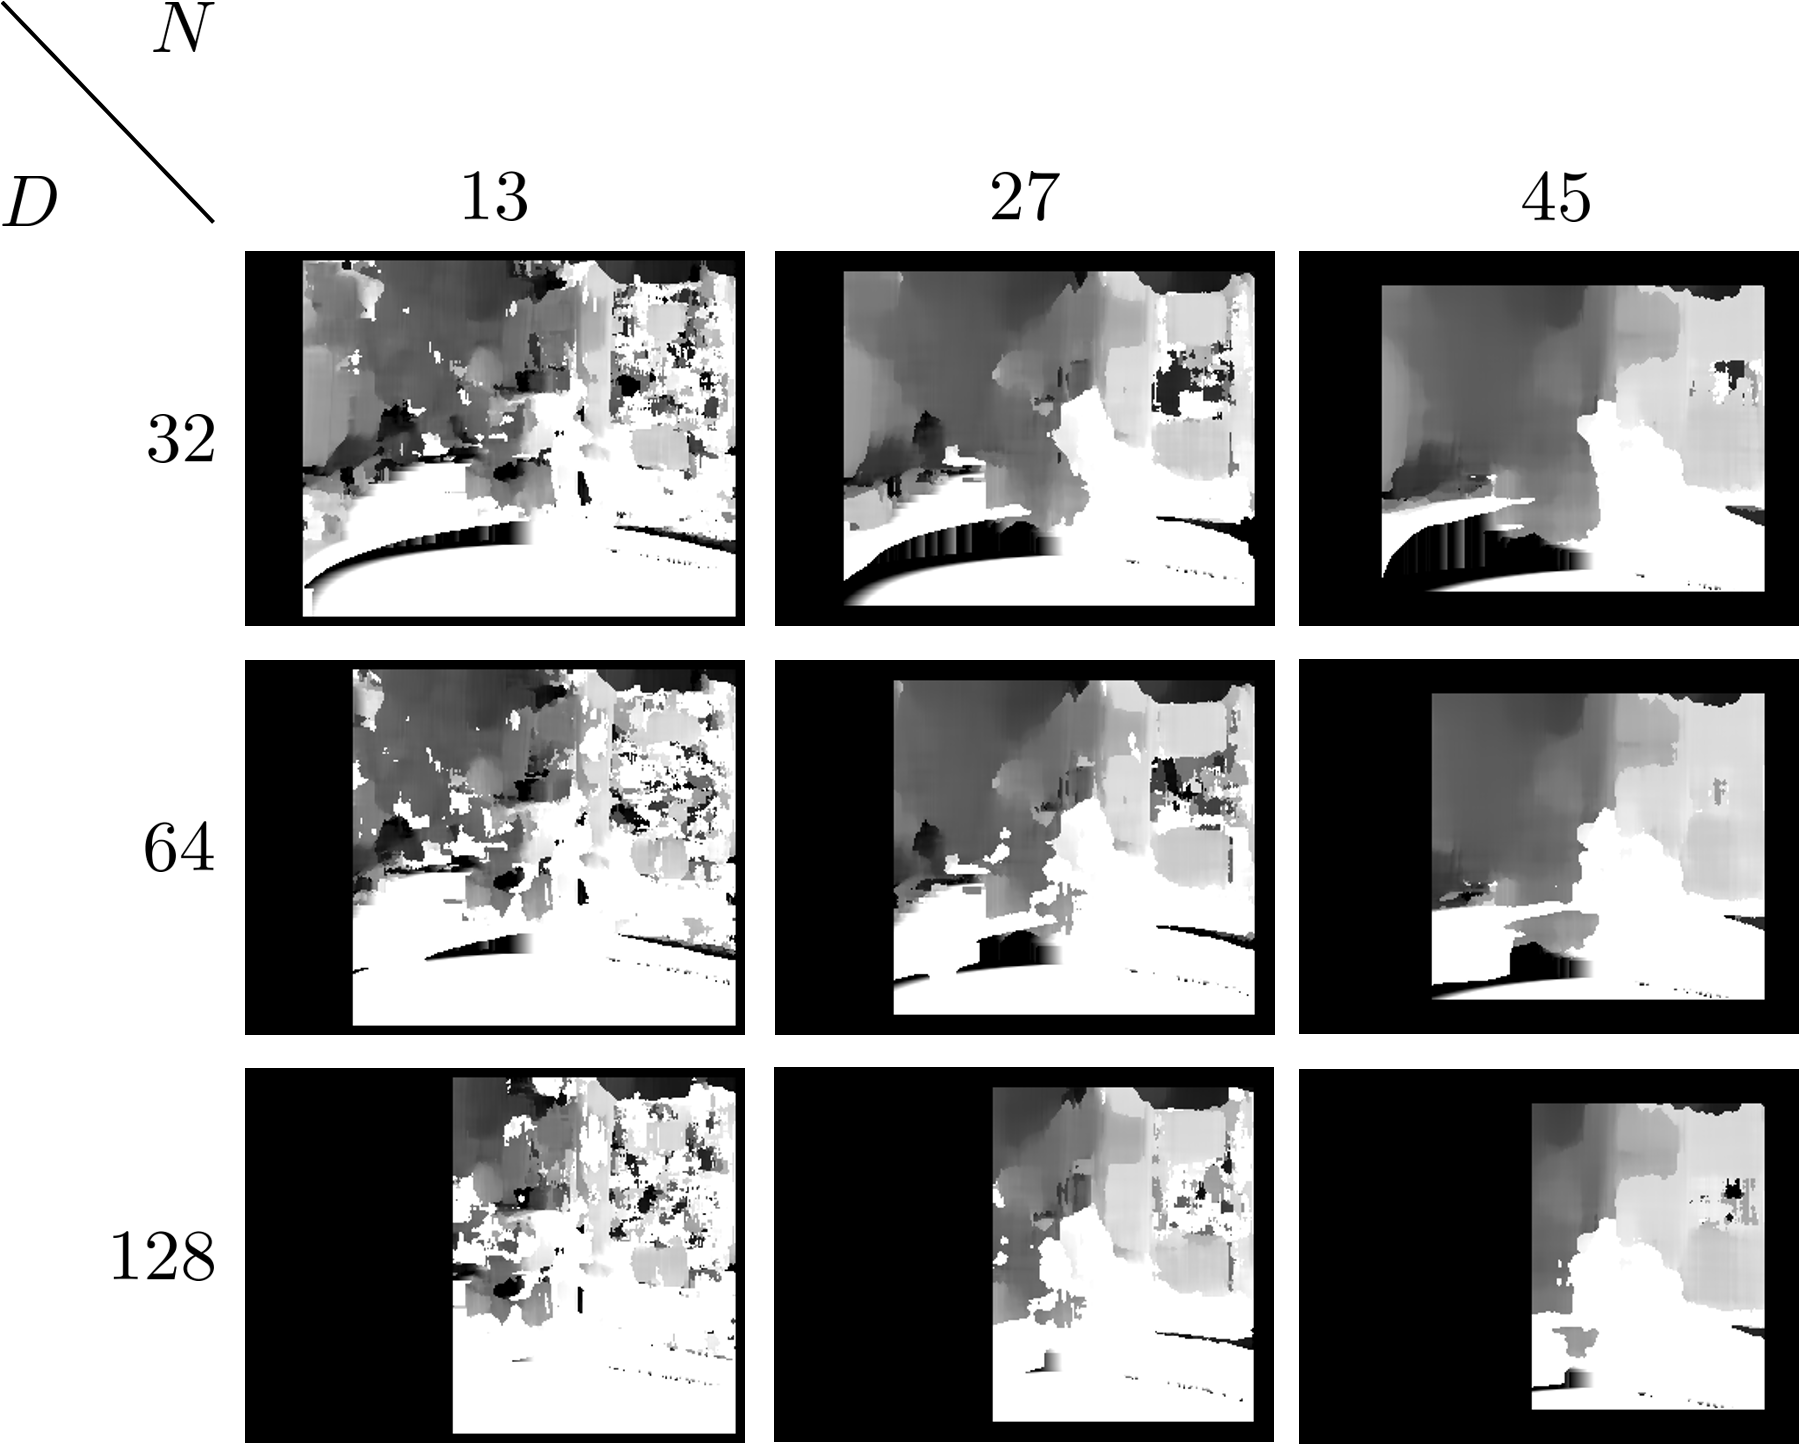
\includegraphics[scale=.2]{chapters/05_experiments/02_autonomous_walking/02_depth_map_parameter_tuning/disp_sad.png}}
	\subcaptionbox{Confidence weighted least squares disparity map. Please refer to figure \ref{fig::324_weighted_least_squares_disparity} and equation \ref{eq::324_wls_final} for the theory.}%
	[.45\linewidth]{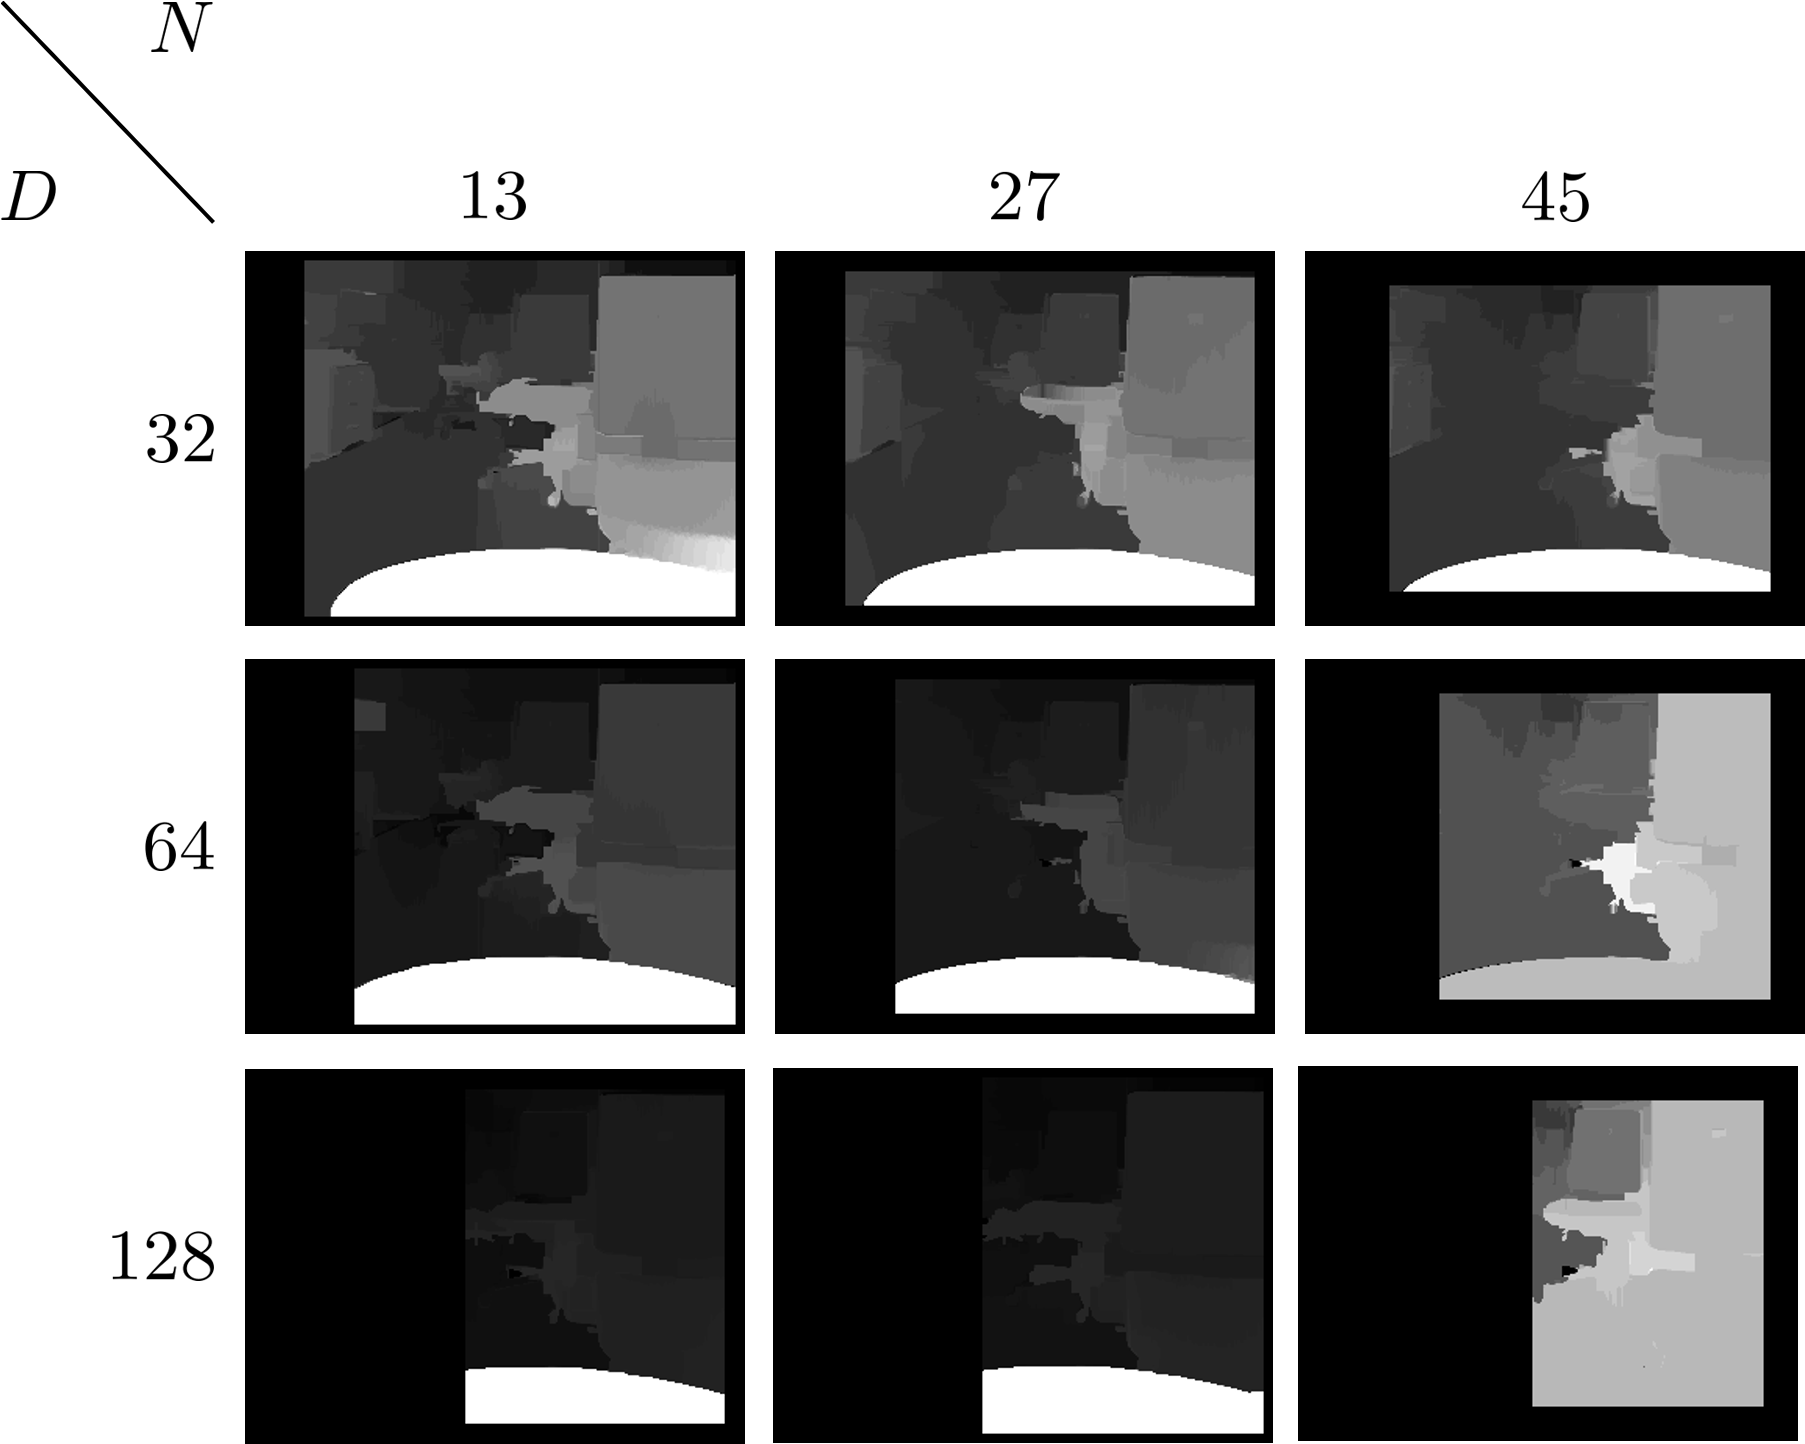
\includegraphics[scale=.2]{chapters/05_experiments/02_autonomous_walking/02_depth_map_parameter_tuning/disp_sad_wls.png}}
	\caption{Left disparity map and confidence weighted least squares disparity for changing SAD window sizes $N$ and number of disparities $D$.}
	\label{fig::522_disp}
\end{figure}
In combination with the confidence weighted least squares filtering, we can observe that most of the noise is already removed (figure \ref{fig::522_disp} (b)), for which it is more import to keep the information close to the images' borders. We therefore chose to set the number of disparities $D=32$, and the windows size $N=13$ in the following. Within these depth maps, the global energy weighting $\lambda$ was set to $10^4$, and the local bilateral filter decay $\sigma$ to $1$, since we observed the best performance for them. The influence of those two parameters is visualized in figure \ref{fig::522_sigma_lambda}. We can see that, in good accordance with the theory, $\sigma$ contributes to the smoothing of the depth map, and that $\lambda$ enforces a change in depth across edges within the RGB images.
\begin{figure}[h]
	\centering
	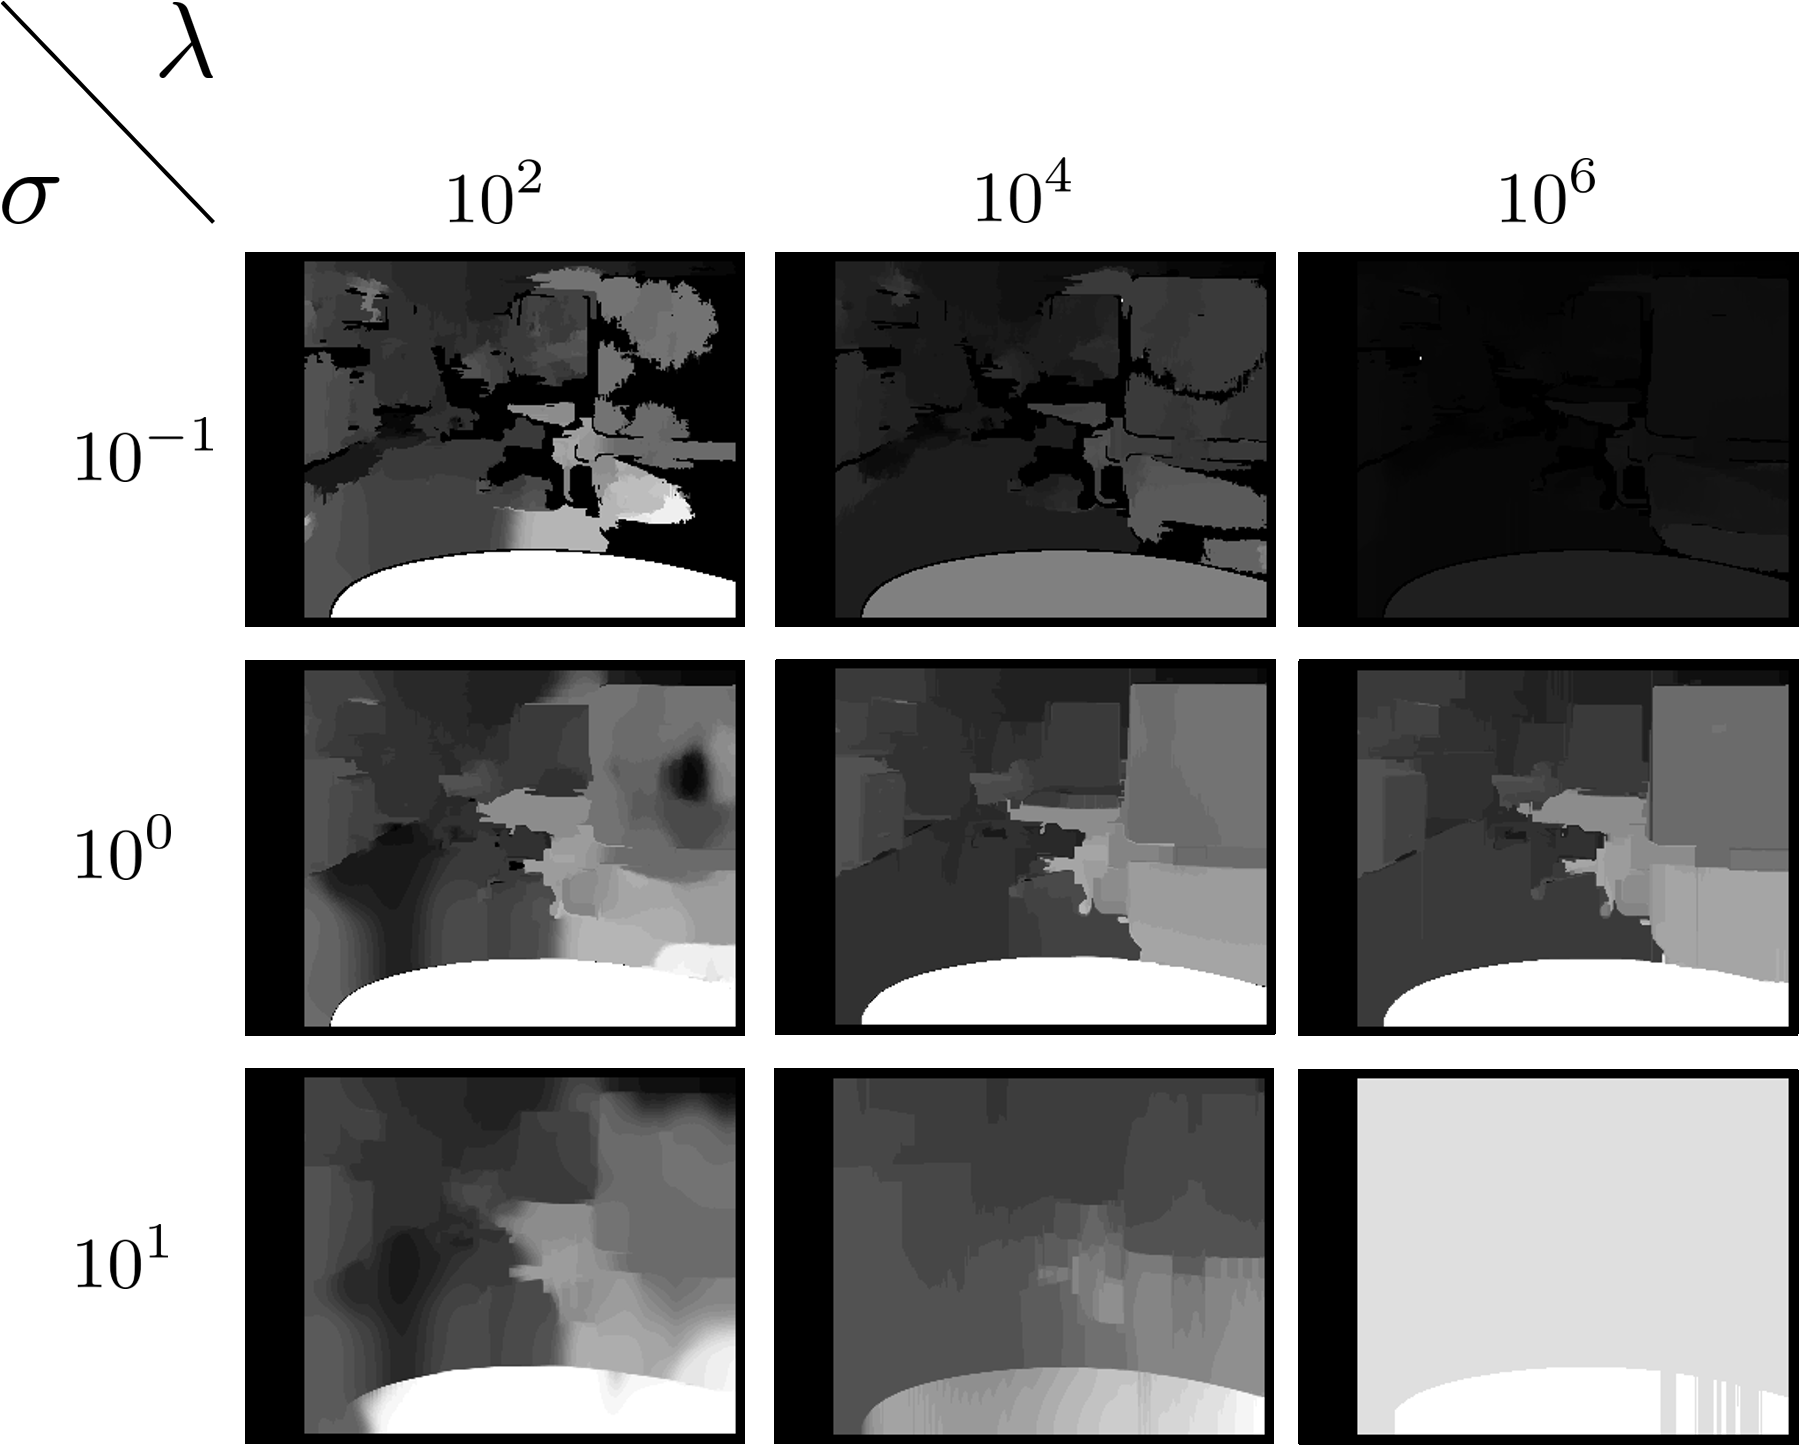
\includegraphics[scale=.2]{chapters/05_experiments/02_autonomous_walking/02_depth_map_parameter_tuning/sigma_lambda.png}
	\caption{Confidence weighted least squares disparity for changing energy weightings $\sigma$ and $\lambda$. Please refer to equations \ref{eq::324_weight} and \ref{eq::324_energy_function} for the theory.}
	\label{fig::522_sigma_lambda}
\end{figure}
\subsection{Data Acquisition and Training}
\label{sec::523_da}
As already pointed out, the task we wanted our neural network to solve was to find a fire extinguisher within a room and then to move towards it. For us to apply behavioral cloning to the task, it was necessary to act according to this policy first, and then to train a neural network on the acquired data. For the data, it is essential to sample homogeneously over the task's distribution. We therefore recorded velocity commands and the corresponding images for 66 distinct epochs. Each of the epochs was designed to reflect different scenarios, among them obstacle avoidance, interaction with humans, walking towards the fire extinguisher, and searching for the fire extinguisher when it was not possible to directly see it. As a result of the observations that we gained from the user controlled walking in section \ref{sec::51_uc}, we restricted the user's policy to only use linear velocities along the x-axis, and angular velocities about the z-axis, since linear velocities along the y-axis revealed to pose an inefficient way of moving the robot. Exemplary samples of the recorded dataset are presented in figure \ref{fig::523_dataset}.
\begin{figure}[h]
	\centering
	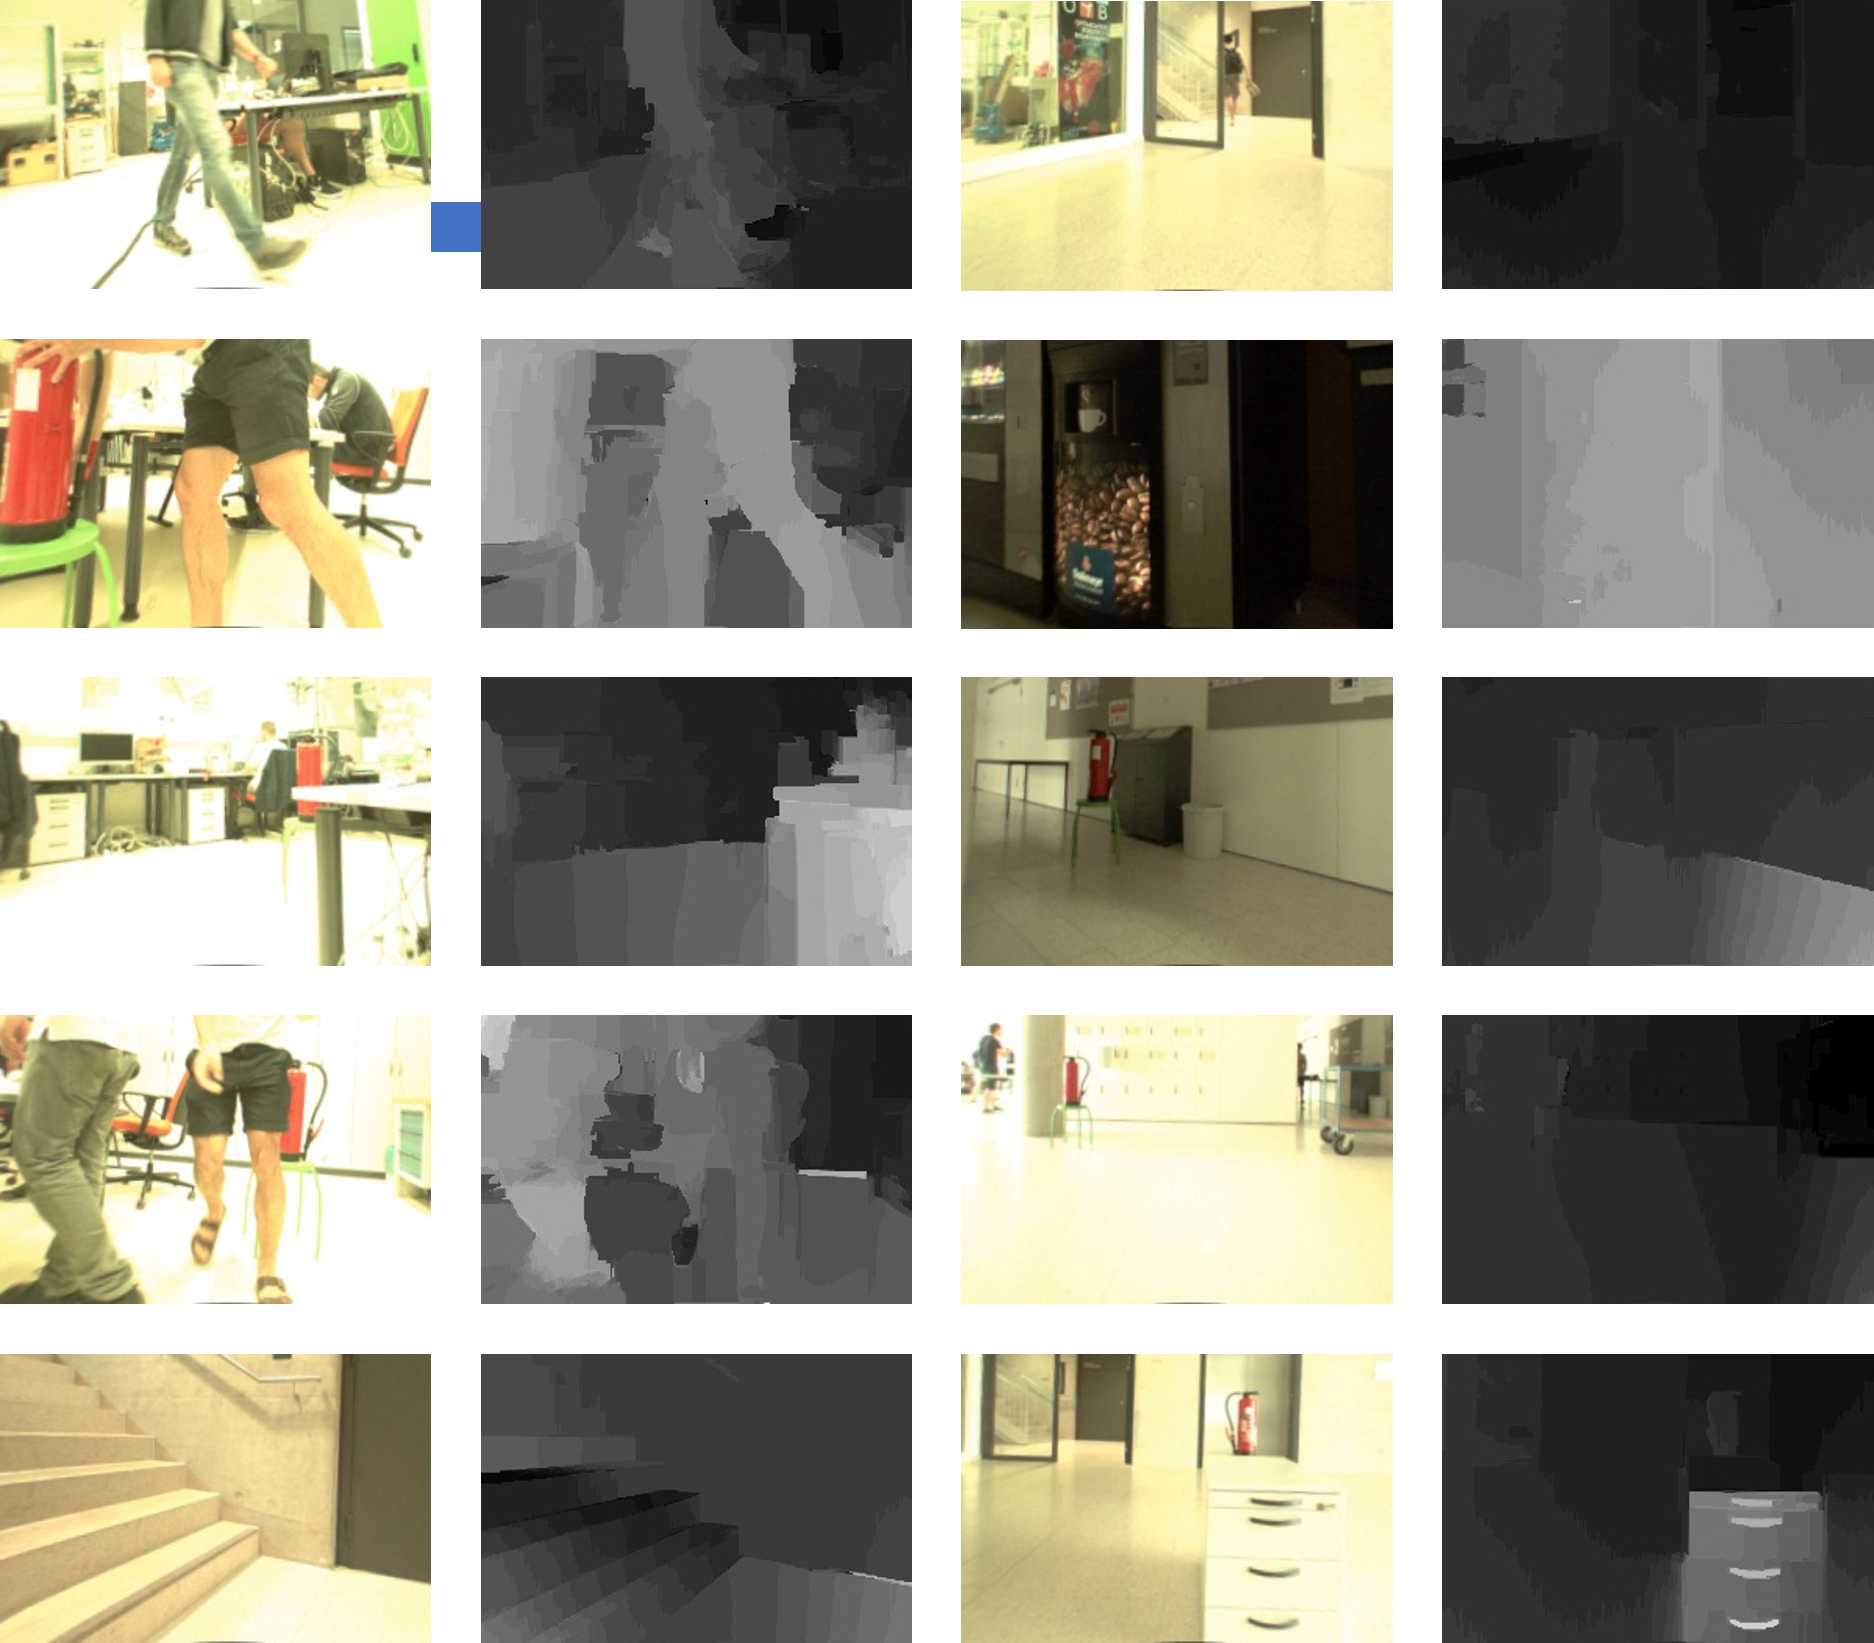
\includegraphics[scale=.4]{chapters/05_experiments/02_autonomous_walking/dataset_diversity.png}
	\caption{Samples of the recorded dataset. The dataset shows a very diverse number of situation for the neural network to learn from.}
	\label{fig::523_dataset}
\end{figure}
It contains 134401 samples in total, which were recorded at a rate of 5 frames per second, and therefore they account for roughly 7.5 hours of data. For each sample, we stored the left camera's RGB view, as well as the confidence weighted least squares disparity map. This lead to a total of 268802 recorded images at a resolution of $240\times320$ pixels, which together make up for $4.7\,\text{GB}$ of data. As a preprocessing step, we cropped regions of the recorded images that do not contain useful information. These regions are firstly caused by deformations that are introduced at the rectification step, as can for example be seen in figure \ref{fig::522_wls_rgb}, and secondly by the depth map's extraction, which results in unknown regions at the image's boarders (figure \ref{fig::522_disp}). The exemplary samples from the dataset (figure \ref{fig::523_dataset}), are already preprocessed, and we can observe how only useful information is kept, in order not to confuse the neural network. To reduce the required amount of GPU memory, we further downscaled the preprocessed images to a size of $60\times80$ pixels, a size at which most of the information is still being kept, and stacked the RBD images with the confidence weighted least squares disparity map to obtain RBGD images. For the training of the neural network, we split the acquired dataset into a train, and a validation set. The training set held a randomly sampled fraction of $90\%$ of all recorded images, while the validation split held the other $10\%$. We only trained the neural network on the training set, and stored the weights that performed best on the validation split, in order to avoid overfitting. Since it has shown very good convergence on our dataset, we chose to use a UNet \cite{ronneberger2015u} as the network architecture, which can be seen in figure \ref{fig::523_unet}.
\begin{figure}[h]
	\centering
	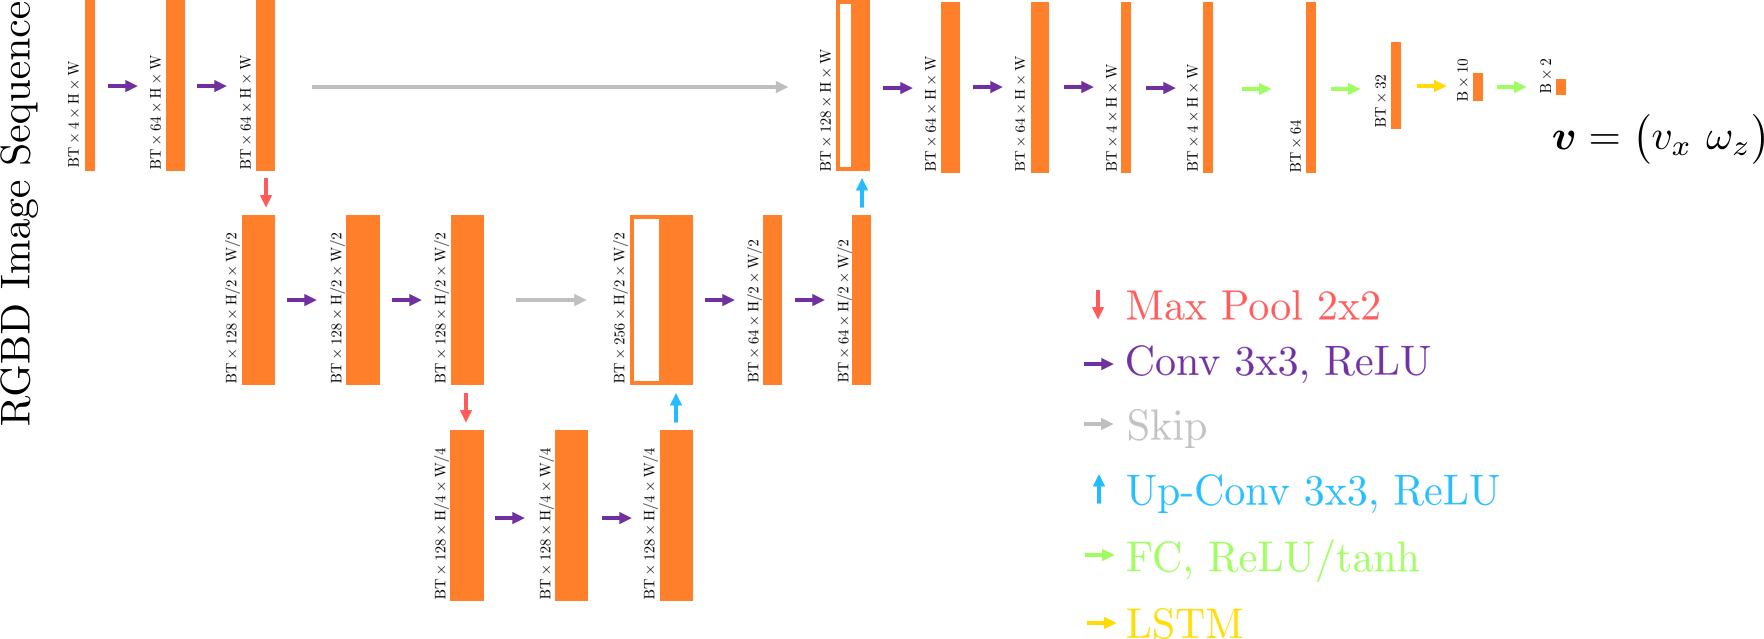
\includegraphics[scale=.5]{chapters/05_experiments/02_autonomous_walking/unet.png}
	\caption{UNet-LSTM network architecture.}
	\label{fig::523_unet}
\end{figure}
The UNet promotes image abstraction capabilities of an auto-encoder that is caused by its bottleneck design, and furthermore shows faster convergence due to its residual connections, which allow the gradient flow to reach deeper layers earlier. Each image that is being forwarded, goes through a number of convolutional layers with rectifying linear unit activation functions, and is subsequently downscaled by max-pooling operations. We repeated this process for two times. Once the most downscaled layer is reached, the weights are being upscaled by simple interpolations again, which simply results in the same resolution that the layers had during the downscaling process. The skip connections then concatenate the shallow with the deep layers to a new layer at each scale, which is then being forwarded further through a number of convolutional layer with rectifying linear units. The nature of the robot's motion, which inherently causes the cameras to periodically move from the left to the right, required us to equip the network architecture by a temporal understanding. We therefore extended the UNet architecture to a novel UNet-LSTM structure. The developed architecture takes up a sequence of consecutive RGBD images, and forwards them through the UNet until it reaches a fully connected regression layer that shall output velocity values in the end. Each image therein creates a signal, from which the LSTM is supposed to only keep the most relevant information. This design helped the network to understand that a fire extinguisher to the left of the image may only be caused by the cameras that are temporally displaced to the right. The final fully connected layer then returns what we use for the loss function, and therefore a velocity. In contrast to the preceding layers, the last fully connected layer uses a hyperbolic tangent function, which restricts the output to a range of $[-1,1]$, which is then being scaled by the velocity that the pattern generator maximally allows. The architecture can be found at the provided \href{https://github.com/mhubii/nmpc_pattern_generator/blob/master/libs/learning/python/unet_model.py}{link}. Due to memory limitations, we trained the network on a sequence length of 5 RGBD images, and a batch size of 32. For the loss, we chose a mean squared error with respect to the most recent velocity command. We used the Adam optimization \cite{kingma2014adam} at a learning $0.001$, and trained for 100 epochs on a TODO, to which we were granted access to. This took us around 48 hours. The loss history is shown in figure \ref{fig::523_loss}, which reveals a good convergence after around 40 epochs.
\begin{figure}[h]
	\centering
	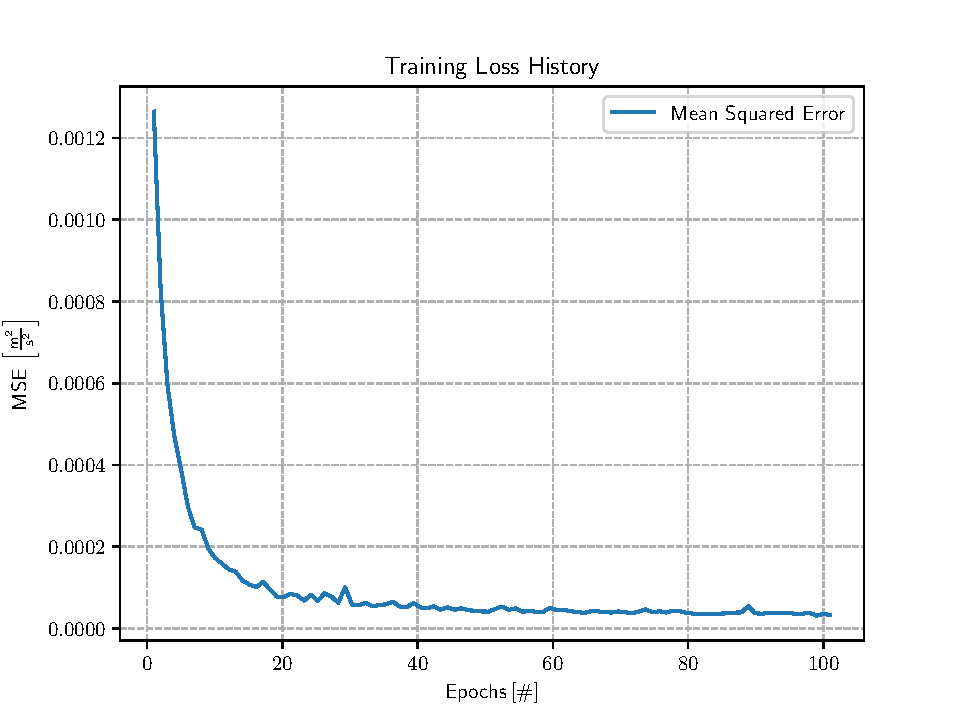
\includegraphics[scale=.4]{chapters/05_experiments/02_autonomous_walking/05_07_19_loss_history.pdf}
	\caption{Mean squared error training loss history.}
	\label{fig::523_loss}
\end{figure}
After training, we generated velocity histograms, as we already did in section \ref{sec::51_uc}, but this time over the whole validation split for both, the ground truth and the predicted behavior, as shown in figure \ref{fig::523_training_dist}. To generate the predictions on the validation split took $4\,\text{ms}$ with a GeForce GTX 1050 for each of the 13341 images on average.
\begin{figure}[h]
	\centering
	\subcaptionbox{Ground truth velocity commands.}%
	[.4\linewidth]{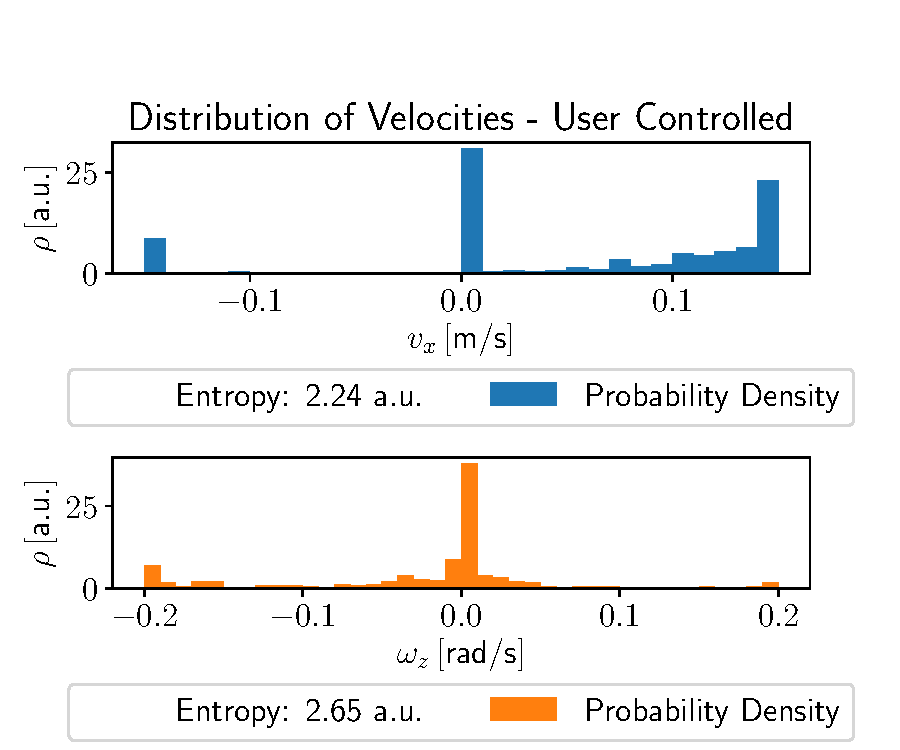
\includegraphics[scale=.35]{chapters/05_experiments/02_autonomous_walking/user_entropy.pdf}}
	\subcaptionbox{Predicted velocity commands.}%
	[.4\linewidth]{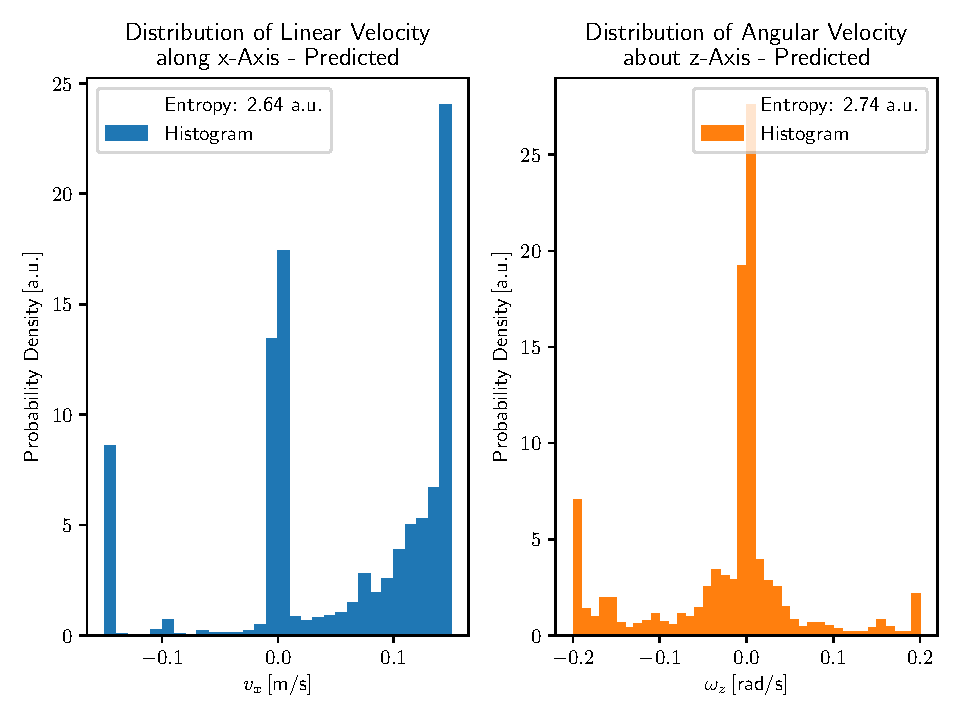
\includegraphics[scale=.35]{chapters/05_experiments/02_autonomous_walking/predicted_entropy_kldivx_0_33_kldivz_0_06_imgs_13441_duration_4_ms.pdf}}
	\caption{Normalized velocity histograms over the validation split.}
	\label{fig::523_training_dist}
\end{figure}
By pure sight, it can already be seen that the network performs well on the validation split, and the Kullback-Leibler divergence $D_\text{KL}$, which measures the distance of probability distributions, enforces this observation further. For the distribution of linear velocities along the x-axis $v_x$, we computed the Kullback-Leibler divergence to be $D^x_\text{KL}=0.33\,\text{a.u.}$, and for the angular velocity about the z-axis $\omega_z$, we obtained $D^z_\text{KL}=0.06\,\text{a.u.}$. Now the beauty within the task at hand lies in the fact that we were not solely dependent on a validation split for performance evaluations, but instead that we simply could run Heicub in a previously unseen test environment. It is the same test environment, which we already introduced in section \ref{sec::51_uc}, and we will evaluate the trained neural network's behavior within it in the next section - Perfomance in Test Environment.
\subsection{Performance in Test Environment}
For the performance benchmarking, we 
\begin{figure}[h]
	\centering
	\subcaptionbox{Straight walk - \href{https://drive.google.com/file/d/1X-RQ9yVLJ9McgeXVoDQhI1uvMJA5o08y/view?usp=sharing}{link}.}%
	[.4\linewidth]{\animategraphics[height=1.2in,loop,autoplay]{20}{chapters/05_experiments/02_autonomous_walking/straight_walk_01/frame-}{001}{033}}
	\subcaptionbox{Curved walk - \href{https://drive.google.com/file/d/1TpT7PUw8cWaUvy1toccXsNO_lQQFlFIS/view?usp=sharing}{link}.}%
	[.4\linewidth]{\animategraphics[height=1.2in,loop,autoplay]{20}{chapters/05_experiments/02_autonomous_walking/curved_walk_02/frame-}{001}{039}}
	\subcaptionbox{Obstacle avoidance - \href{https://drive.google.com/file/d/1DlO8Rd6AiBPrHKbTIgI12d2ySaTvMJ3S/view?usp=sharing}{link}.}%
	[.4\linewidth]{\animategraphics[height=1.2in,loop,autoplay]{20}{chapters/05_experiments/02_autonomous_walking/obstacle_walk_02/frame-}{001}{017}}
	\subcaptionbox{Environment scanning - \href{https://drive.google.com/file/d/1QmtltYTwoXMzHoUA8knA2FEpMsaud0QD/view?usp=sharing}{link}.}%
	[.4\linewidth]{\animategraphics[height=1.2in,loop,autoplay]{20}{chapters/05_experiments/02_autonomous_walking/out_of_sight_walk_01/frame-}{001}{075}}
	\caption{Heicub's behavior in the test environment for benchmarking tasks.}
	\label{fig::524_aw_gif_basic}
\end{figure} 
\begin{figure}[h]
	\centering
	\subcaptionbox{Straight walk - dynamic balance.}%
	[.4\linewidth]{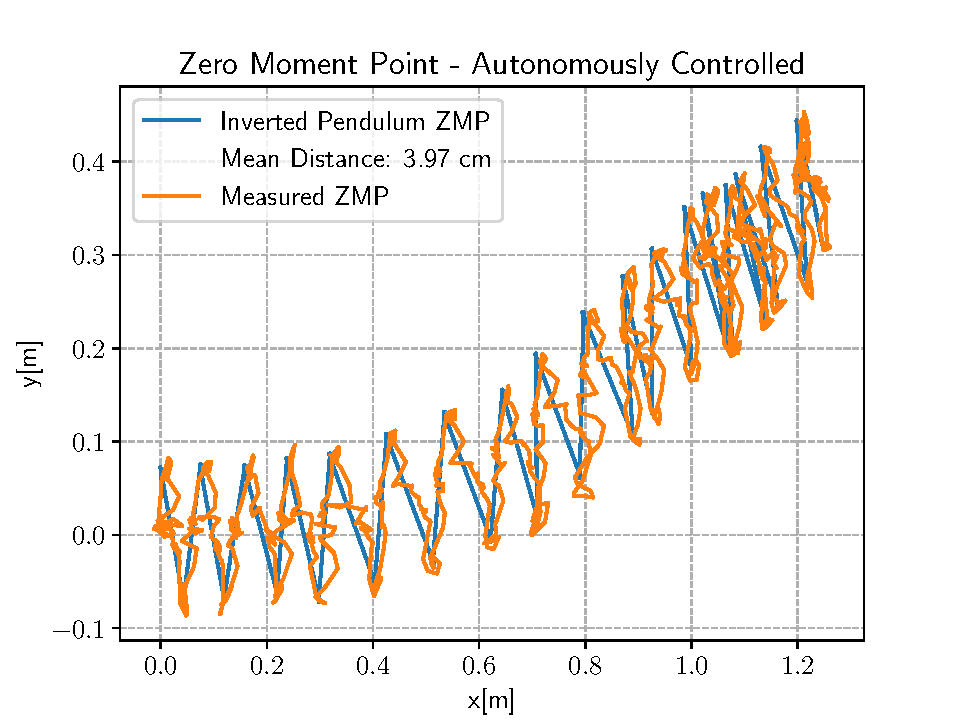
\includegraphics[scale=.35]{chapters/05_experiments/02_autonomous_walking/straight_walk_01_zmp.pdf}}
	\subcaptionbox{Straight walk - behavior.}%
	[.4\linewidth]{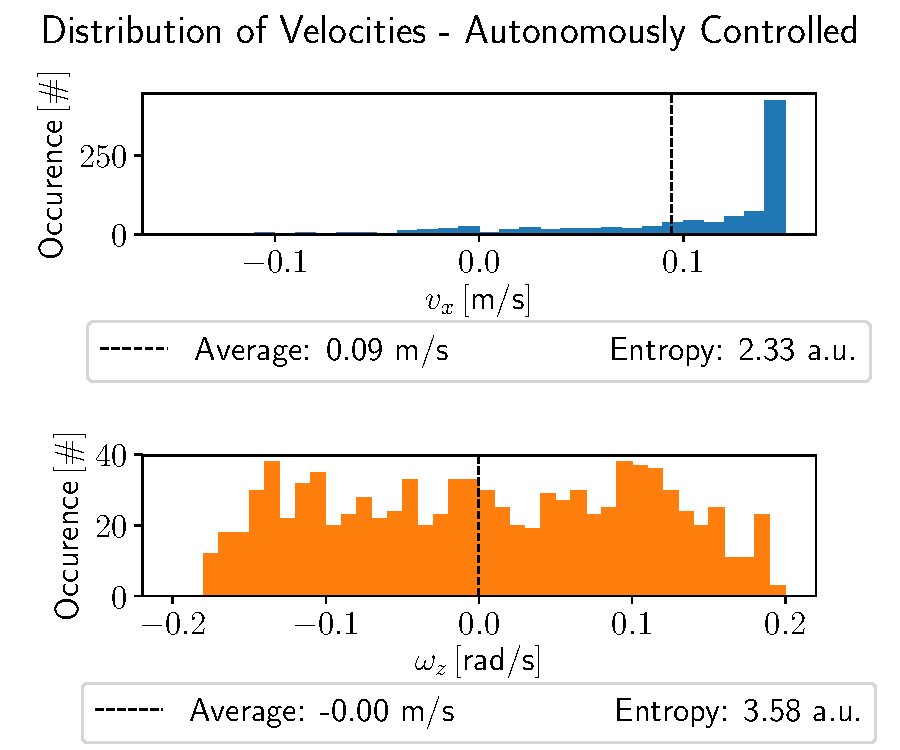
\includegraphics[scale=.35]{chapters/05_experiments/02_autonomous_walking/straight_walk_01_entropy.pdf}}
	\subcaptionbox{Curved walk - dynamic balance.}%
	[.4\linewidth]{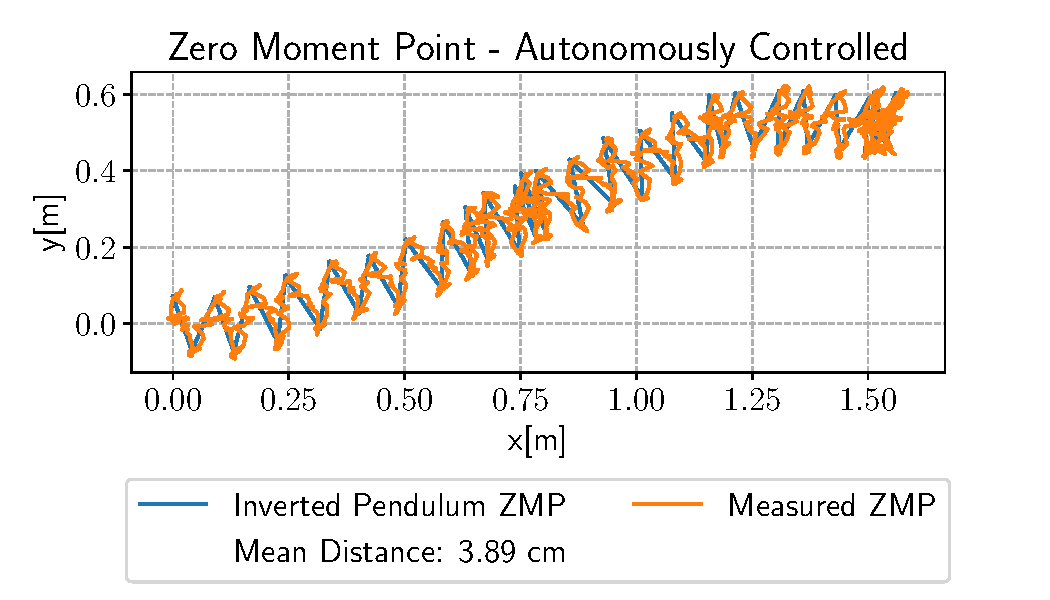
\includegraphics[scale=.35]{chapters/05_experiments/02_autonomous_walking/curved_walk_01_zmp.pdf}}
	\subcaptionbox{Curved walk - behavior.}%
	[.4\linewidth]{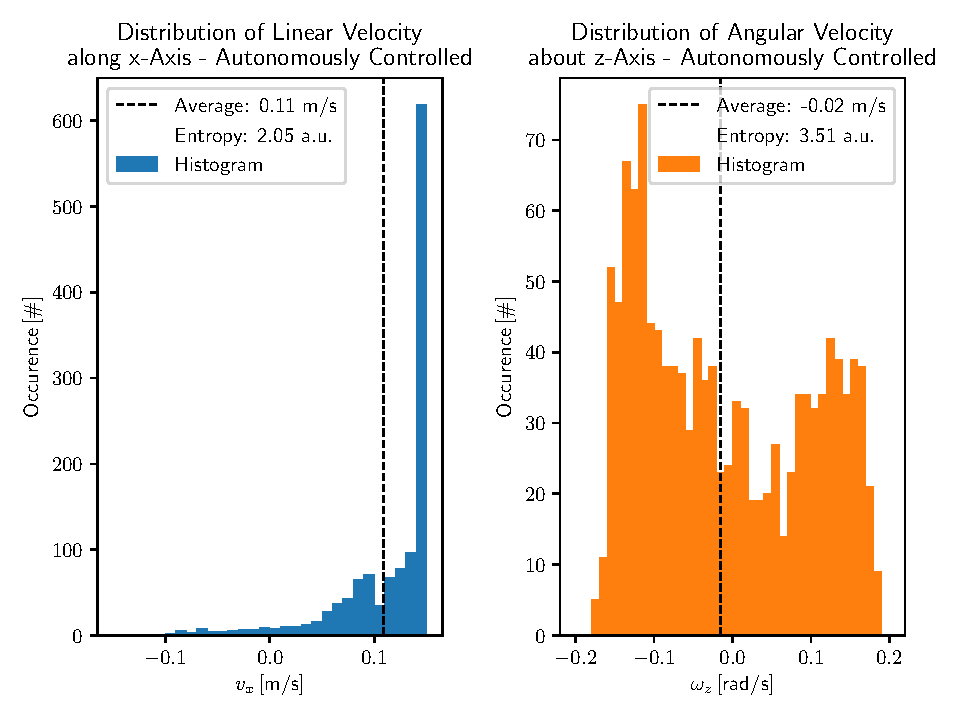
\includegraphics[scale=.35]{chapters/05_experiments/02_autonomous_walking/curved_walk_01_entropy.pdf}}
	\subcaptionbox{Obstacle avoidance - dynamic balance.}%
	[.4\linewidth]{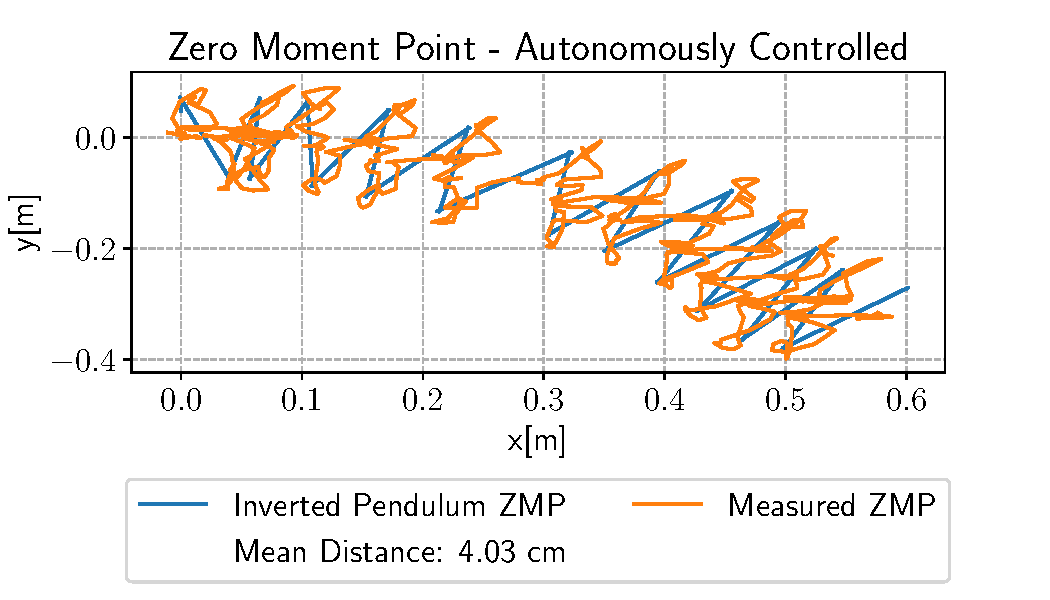
\includegraphics[scale=.35]{chapters/05_experiments/02_autonomous_walking/obstacle_walk_02_zmp.pdf}}
	\subcaptionbox{Obstacle avoidance - behavior.}%
	[.4\linewidth]{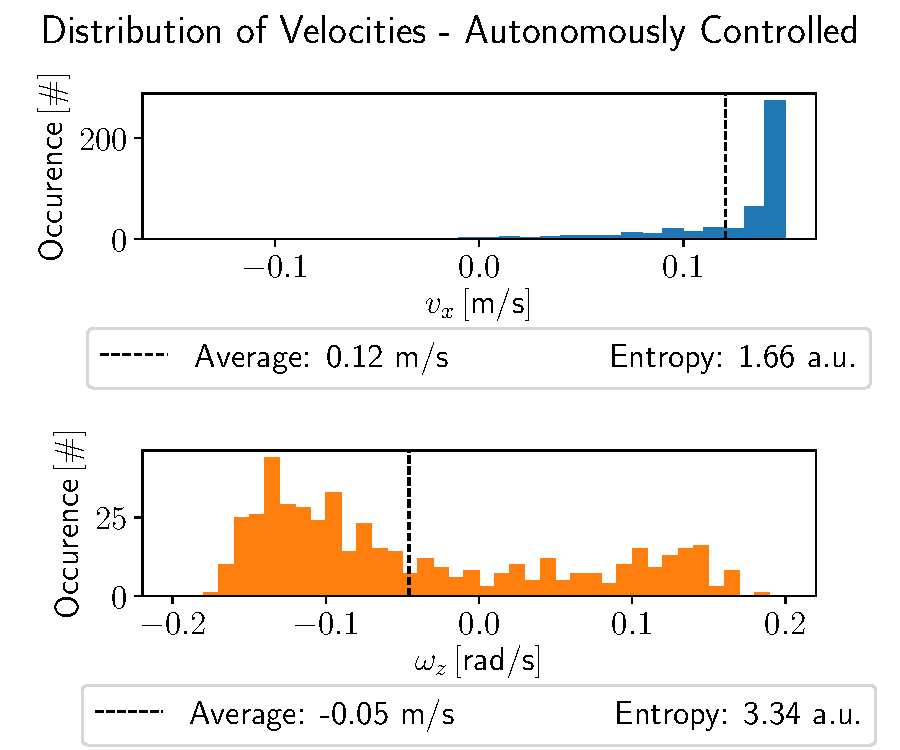
\includegraphics[scale=.35]{chapters/05_experiments/02_autonomous_walking/obstacle_walk_02_entropy.pdf}}
	\subcaptionbox{Environment scanning - dynamic balance.}%
	[.4\linewidth]{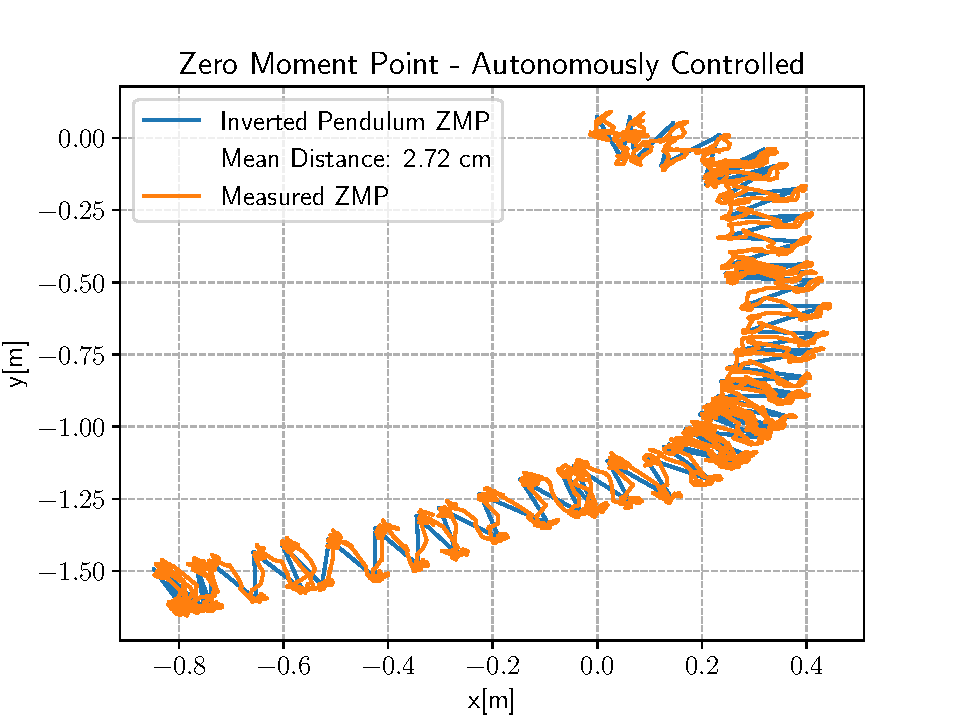
\includegraphics[scale=.35]{chapters/05_experiments/02_autonomous_walking/out_of_sight_walk_01_zmp.pdf}}
	\subcaptionbox{Environment scanning - behavior.}%
	[.4\linewidth]{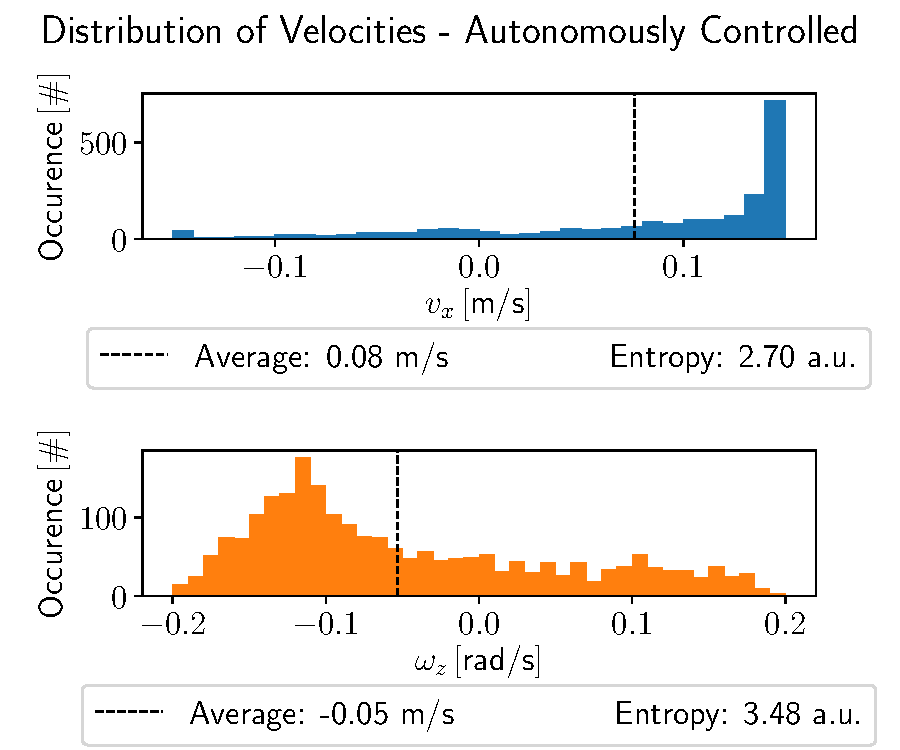
\includegraphics[scale=.35]{chapters/05_experiments/02_autonomous_walking/out_of_sight_walk_01_entropy.pdf}}
	\caption{Heicub's performance under the control of the presented neural network for benchmarking tasks.}
	\label{fig::524_aw_basic}
\end{figure} 
\begin{figure}[h]
	\centering
	\subcaptionbox{Dynamic environment - \href{https://drive.google.com/file/d/1zm-9apobNmsXAcLXB5e9lGqIU7NMHzVl/view?usp=sharing}{link}.}%
	[.4\linewidth]{\animategraphics[height=1.2in,loop,autoplay]{20}{chapters/05_experiments/02_autonomous_walking/dynamic_walk_01/frame-}{001}{031}}
	\subcaptionbox{Semantic understanding - \href{https://drive.google.com/file/d/1VQIEChA61GDxm-rLf8pfOxCgXeJhuFG9/view?usp=sharing}{link}.}%
	[.4\linewidth]{\animategraphics[height=1.2in,loop,autoplay]{20}{chapters/05_experiments/02_autonomous_walking/semantic_walk_01/frame-}{001}{046}}
	\caption{Heicub's behavior in the test environment for additional tasks.}
\label{fig::524_aw_gif_additional}
\end{figure} 
\begin{figure}[h]
	\centering
	\subcaptionbox{Dynamic environment - dynamic balance.}%
	[.4\linewidth]{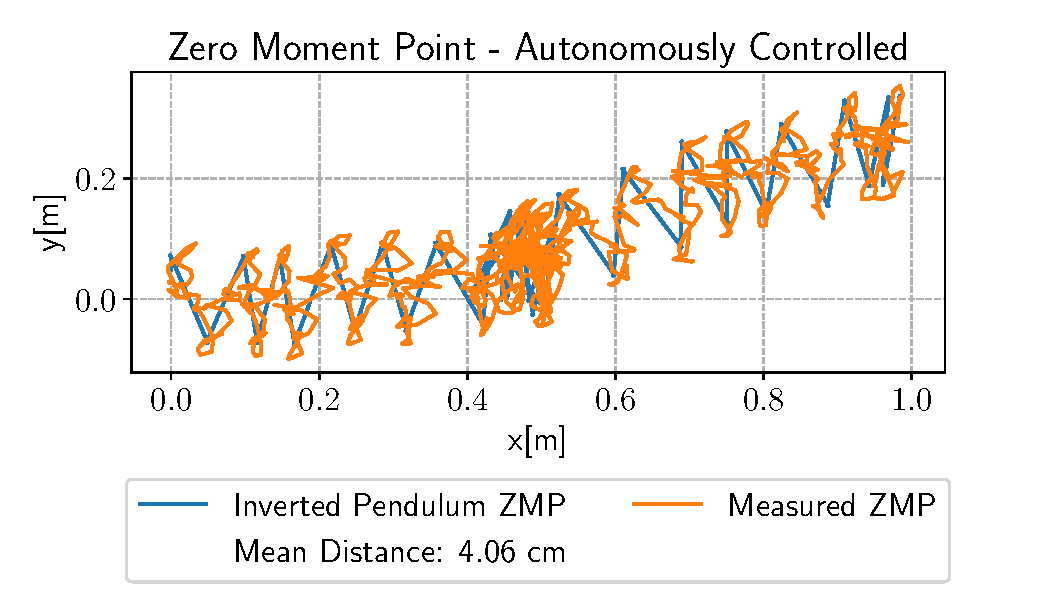
\includegraphics[scale=.35]{chapters/05_experiments/02_autonomous_walking/dynamic_walk_01_zmp.pdf}}
	\subcaptionbox{Dynamic environment - behavior.}%
	[.4\linewidth]{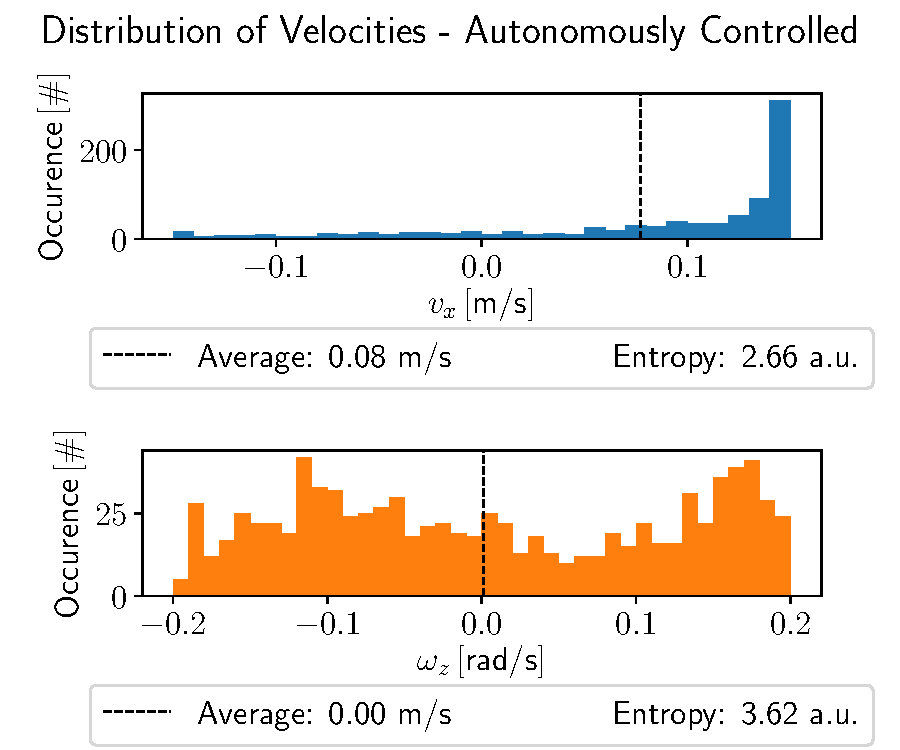
\includegraphics[scale=.35]{chapters/05_experiments/02_autonomous_walking/dynamic_walk_01_entropy.pdf}}
	\subcaptionbox{Semantic understanding - dynamic balance.}%
	[.4\linewidth]{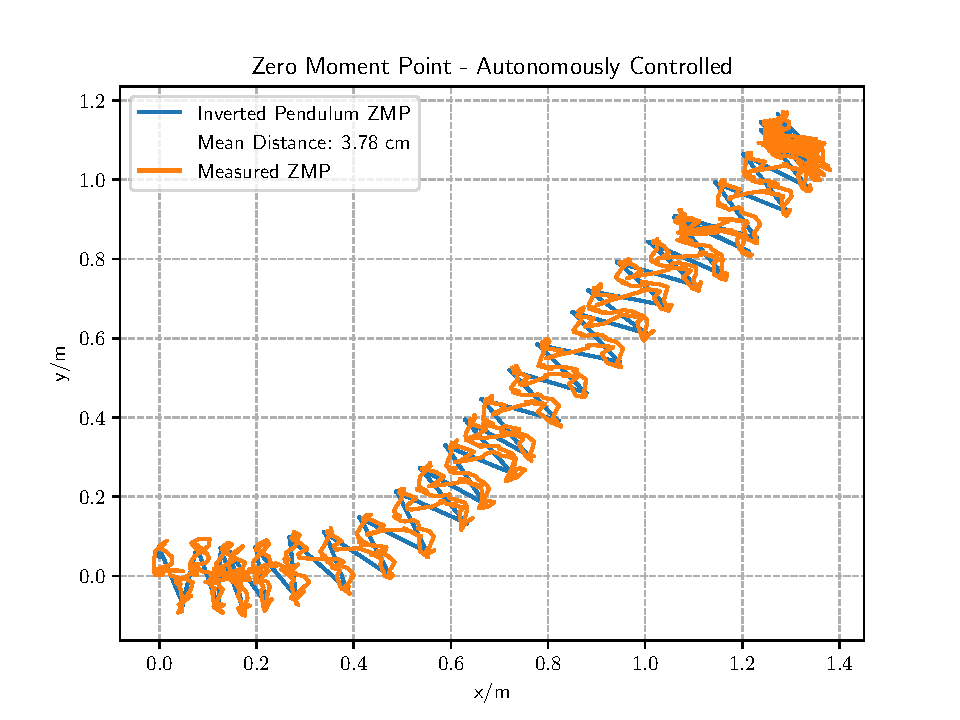
\includegraphics[scale=.35]{chapters/05_experiments/02_autonomous_walking/semantic_walk_01_zmp.pdf}}
	\subcaptionbox{Semantic understanding - behavior.}%
	[.4\linewidth]{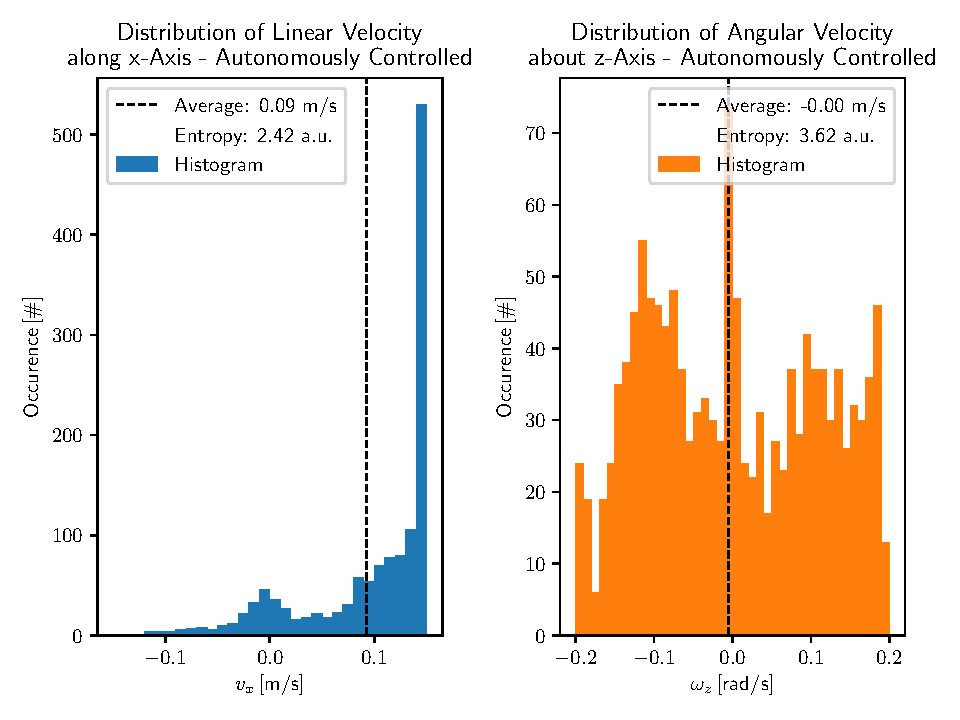
\includegraphics[scale=.35]{chapters/05_experiments/02_autonomous_walking/semantic_walk_01_entropy.pdf}}
	\caption{Heicub's performance under the control of the presented neural network for additional tasks.}
	\label{fig::524_aw_additional}
\end{figure}
\begin{figure}[h]
	\centering
	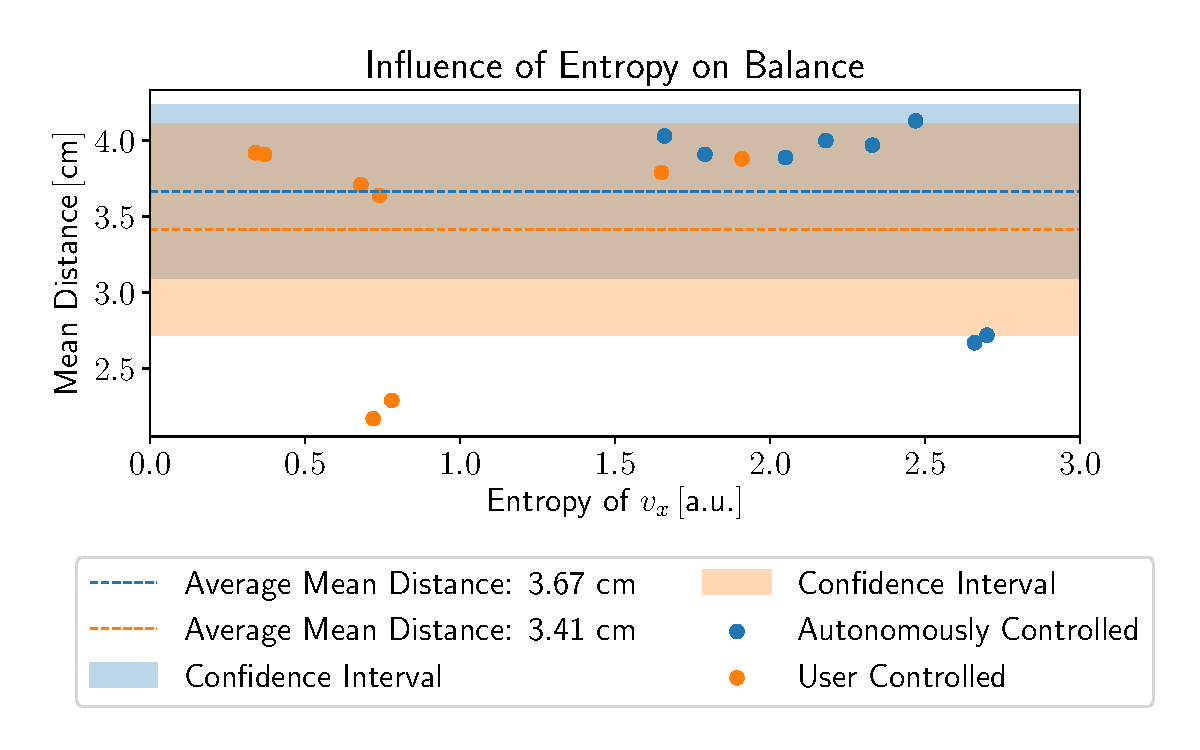
\includegraphics[scale=.5]{chapters/05_experiments/02_autonomous_walking/entropy_against_balance.pdf}
	\caption{Influence of entropic commands onto Heicub's dynamic balance.}
	\label{fig::524_entropy_balance}
\end{figure}
meanaw 3.67, meanuc 3.41, stdaw 0.56, stduc 0.69
\subsection{Proximal Policy Optimization}
